\section{Performance}
\label{sec:Performance}

  A high statistics Monte Carlo simulation was performed in order to estimate the reconstruction efficiency and resolution of the implemented track-finding and track-fitting algorithms. It was necessarily Monte Carlo based in order to compare the reconstructed events to the simulated truth, thereby highlighting any inefficiencies and inaccuracies within the algorithms, without any additional noise or biases.

  The fitted transverse positions, $(x,y)$, and momenta, $(p_x, p_y, p_z)$, were compared against the the Monte Carlo truth on an event-by-event basis. The reconstructed events were not subject to any cuts or additional requirements over those of real data reconstruction. The Monte Carlo truth data was determined from the simulated track information, which was stored at every tracker plane to permit a direct comparison to the reconstructed data. All data sets were compared at the tracker reference surface, the designated measurement location with the MICE cooling channel.

  An artificial beam was generated with uniform distributions in both the longintudinal and transverse momenta. This was to ensure that the results were not biased by the incoming beam distribution, and that the full reconstructable phase space was probed with equal statistics.

  \subsection{Track Finding Efficiency}
  \label{sec:performance:track_finding}

  For every simulated event, the number of expected tracks was calculated from the Monte Carlo truth. If the simulated track crossed enough tracker planes to create a sufficient number of spacepoints (3 for straight tracks and 4 for helical tracks), a reconstructed track was expected. The reconstructed tracks were then compared for each tracker and compared to the expected track parameters. The efficiency of track finding as a function of the true longtudinal and transverse momenta is shown in figure~\ref{fig:track_efficiency}.

  \begin{figure}[p]
    \centering
    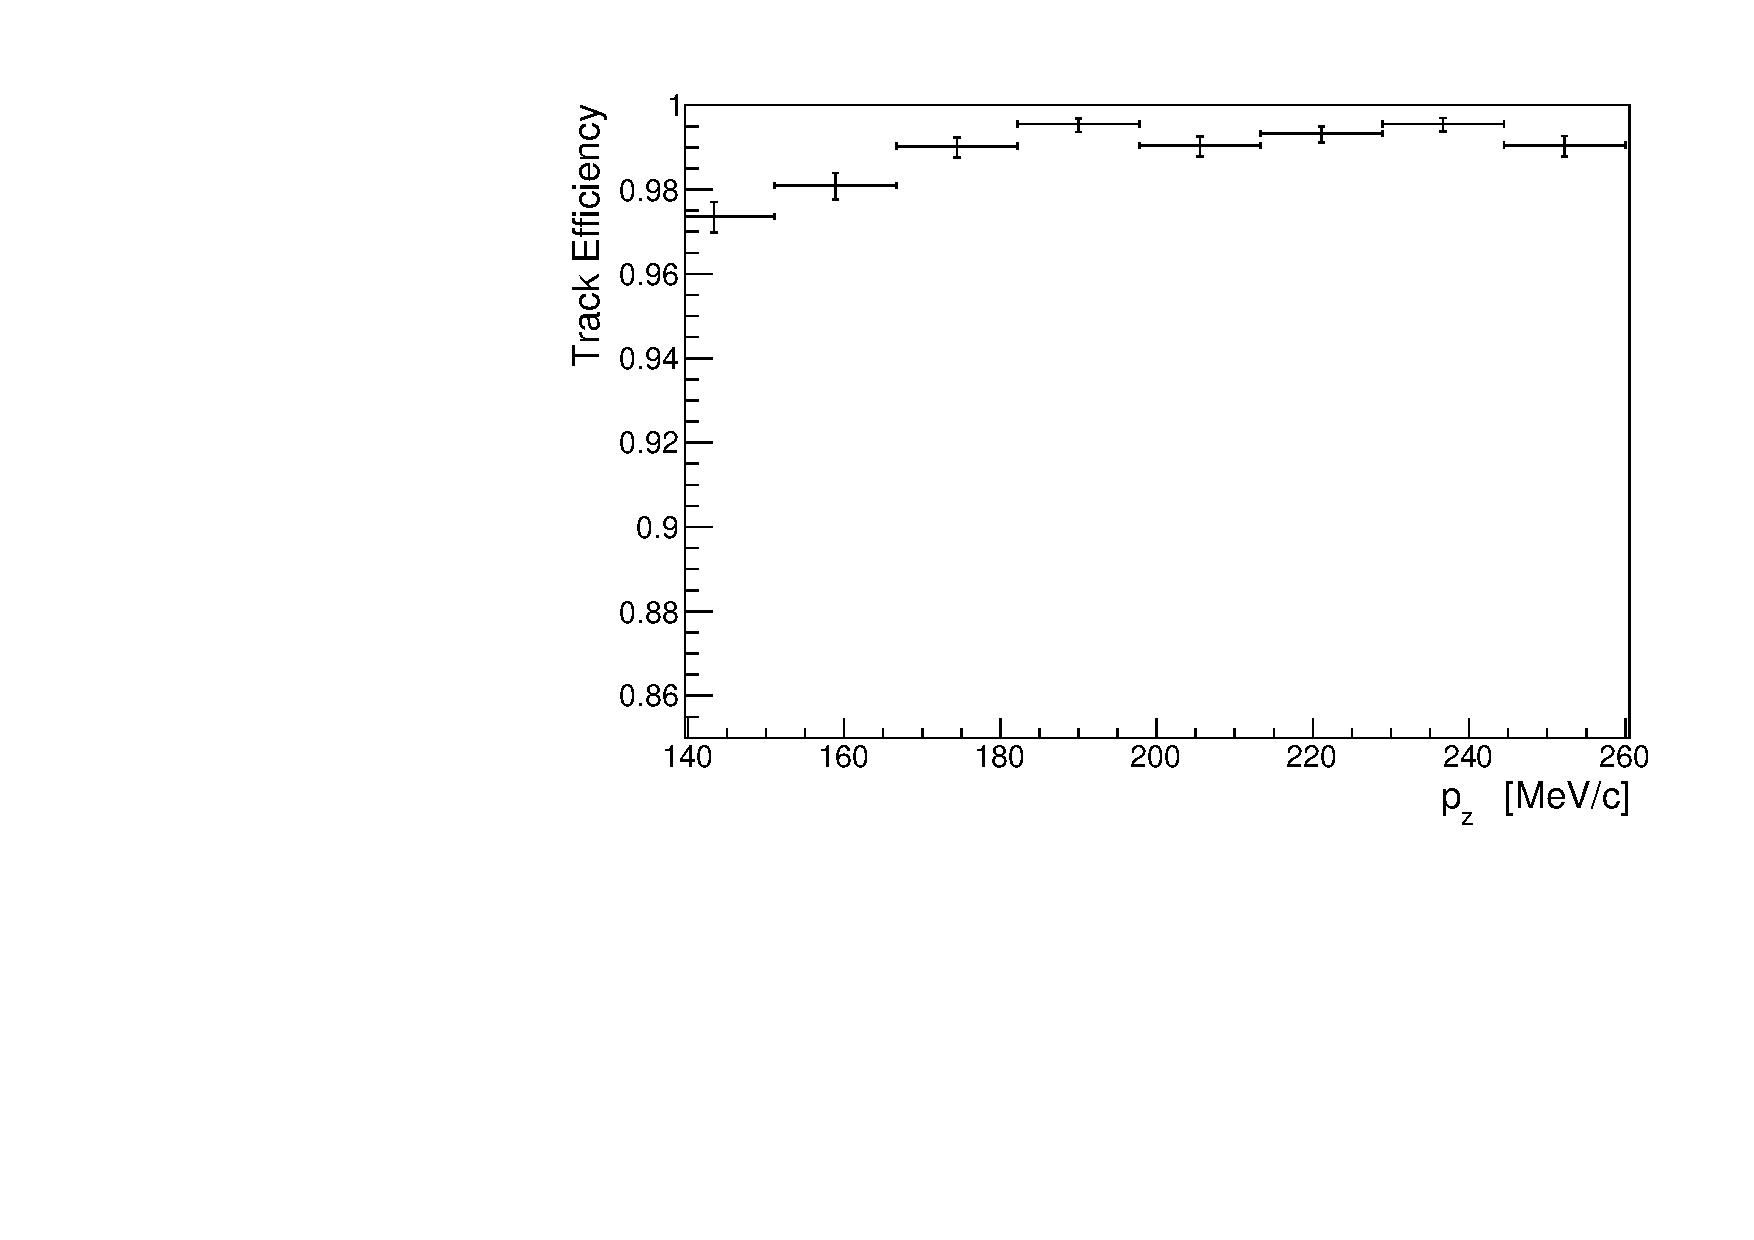
\includegraphics[width=0.45\textwidth, angle=0]{08-Performance/upstream_pz_track_efficiency.pdf}
    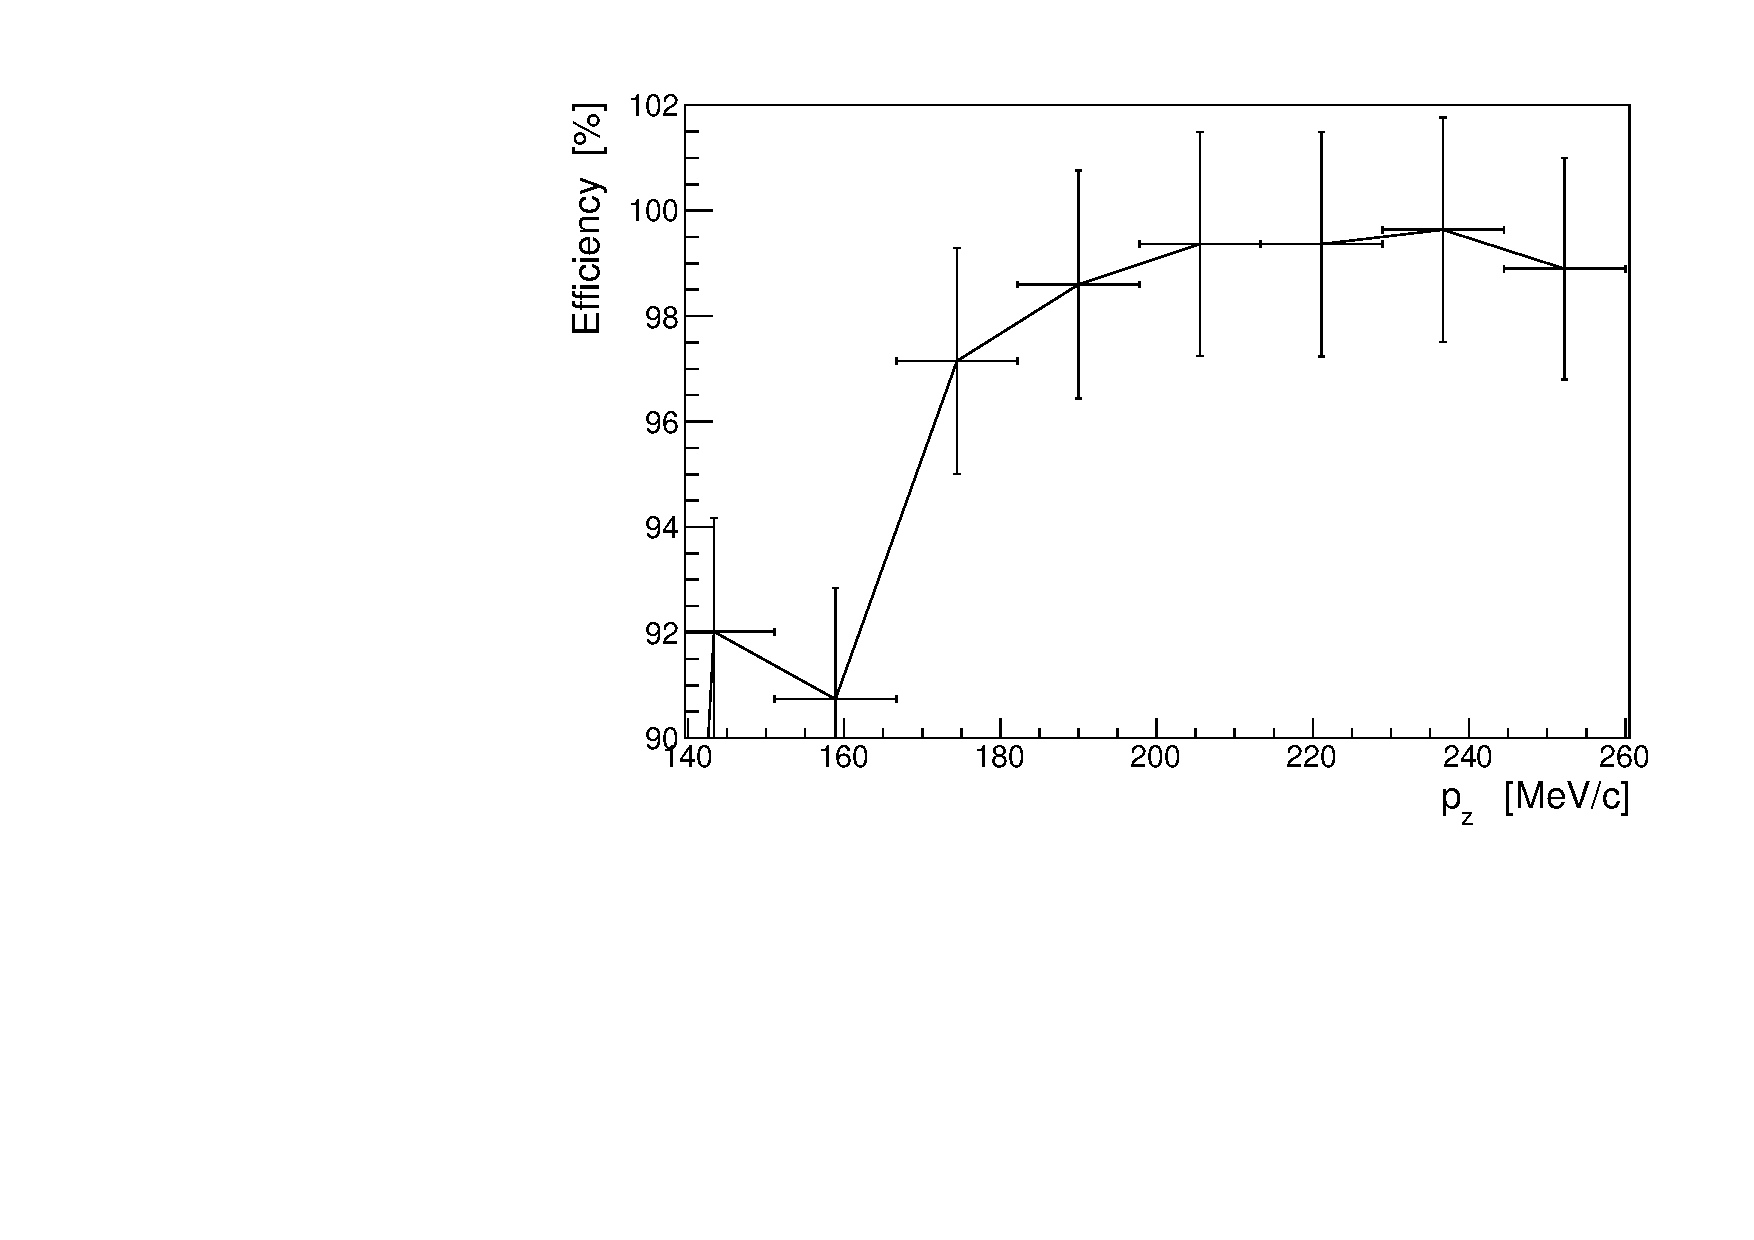
\includegraphics[width=0.45\textwidth, angle=0]{08-Performance/downstream_pz_track_efficiency.pdf}\\
    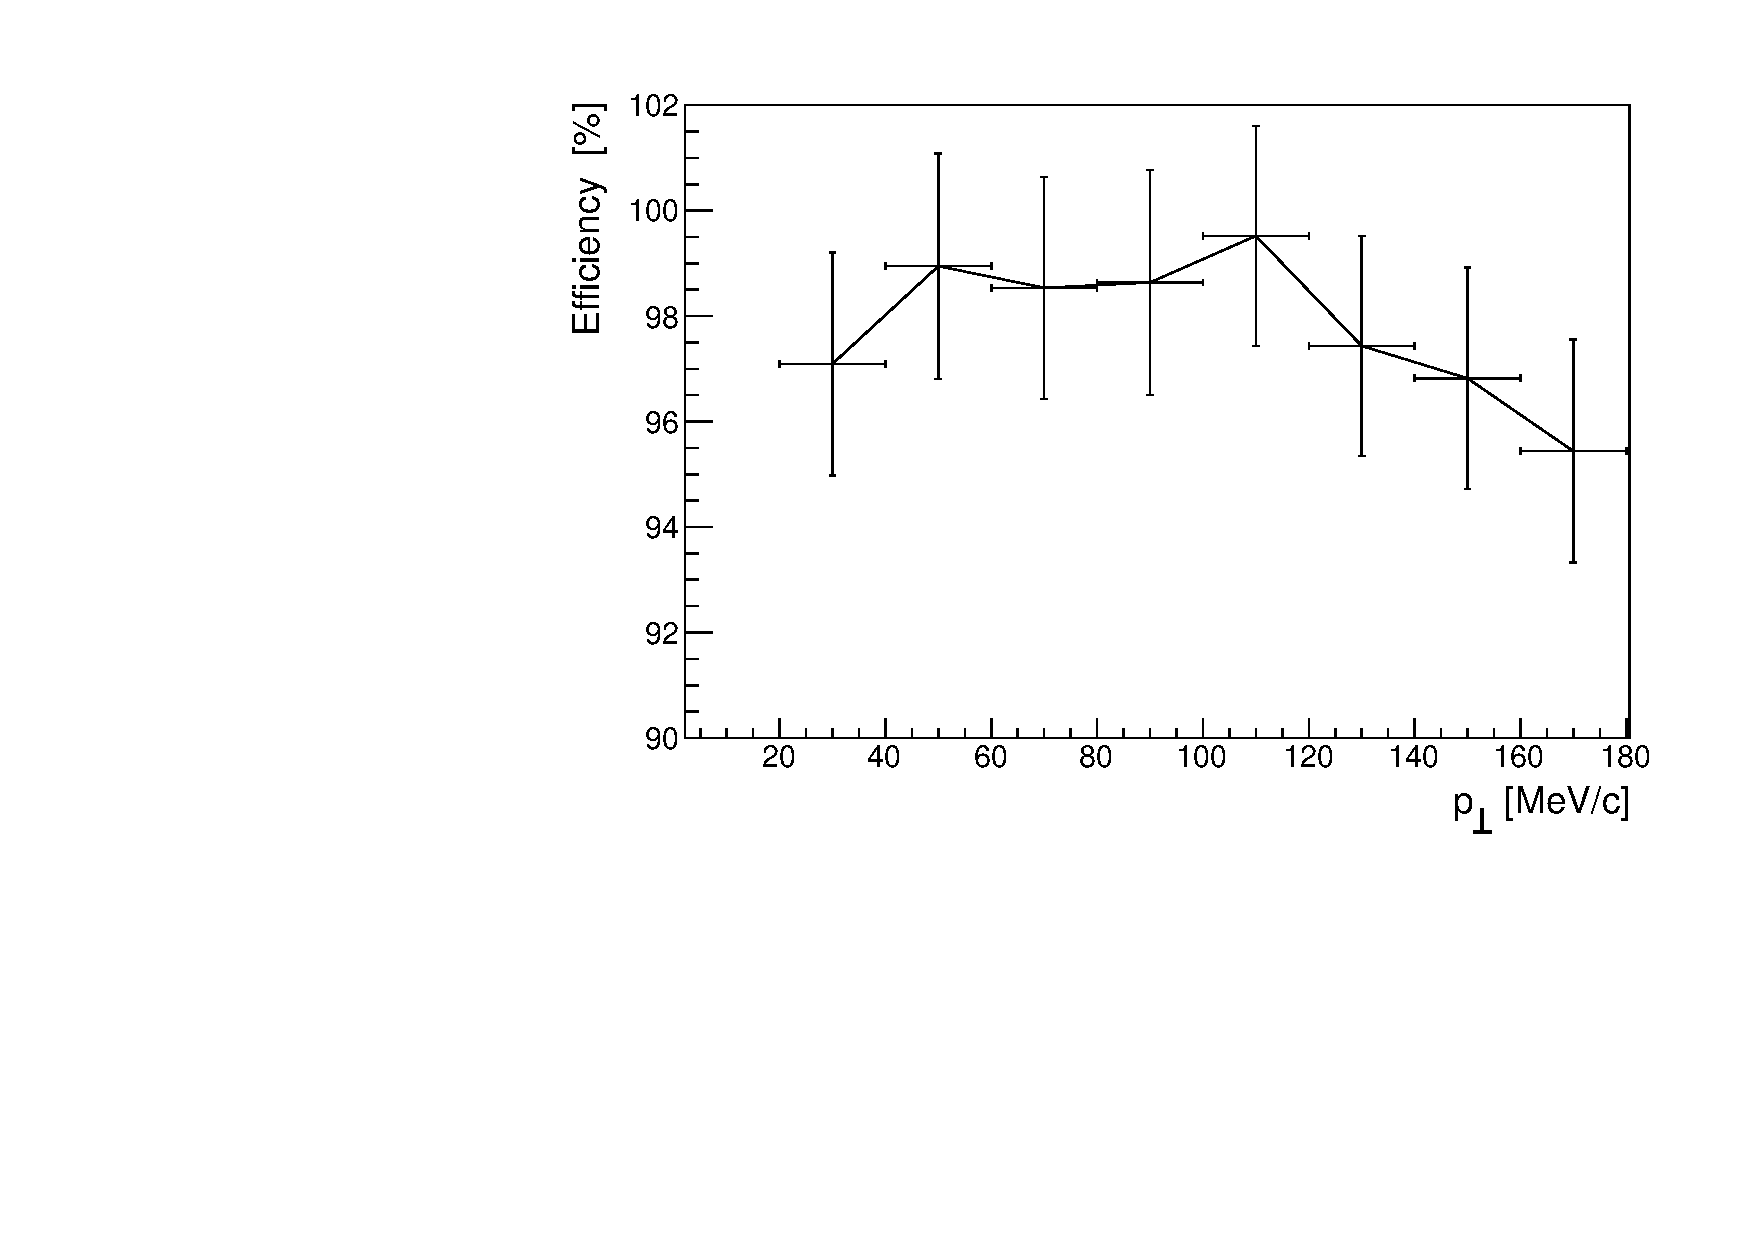
\includegraphics[width=0.45\textwidth, angle=0]{08-Performance/upstream_pt_track_efficiency.pdf}
    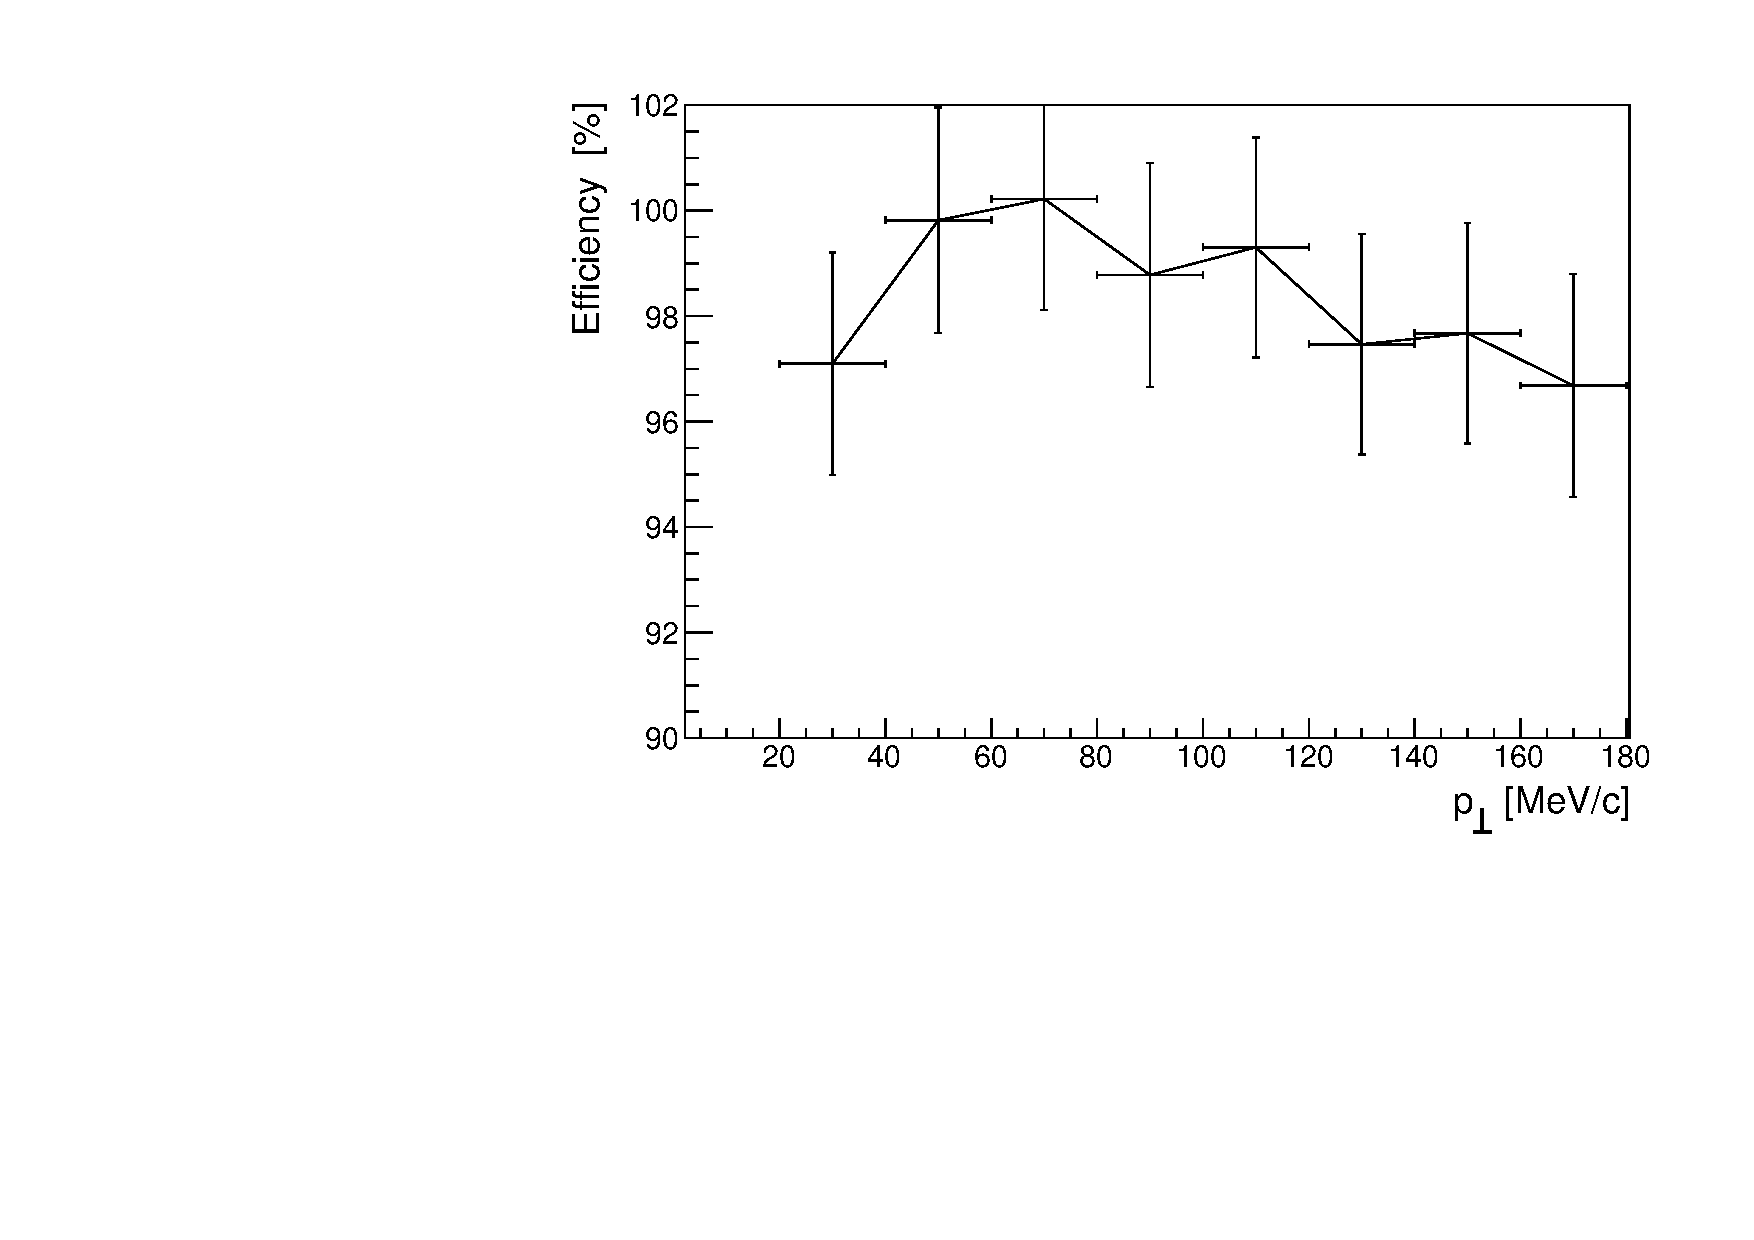
\includegraphics[width=0.45\textwidth, angle=0]{08-Performance/downstream_pt_track_efficiency.pdf}
    \caption{\label{fig:track_efficiency} The efficiency of reconstructing tracks in the upstream (left) and downstream (right) trackers as a function of the simulated longitudinal (top) and transverse (bottom) momentum.}
  \end{figure}

  Once the the Monte Carlo tracks have been identified, the expected number of trackpoints can be calculated by examining the number of tracker planes that the simulated track crossed. Comparing the number of trackpoints in each reconstructed track to the expected number for each simulated track permits the efficiency of finding the correct number of trackpoints to be calculated. Figure~\ref{fig:tp_efficiency} shows the trackpoint finding efficiency as a function of longitudinal and transverse momenta.

  \begin{figure}[p]
    \centering
    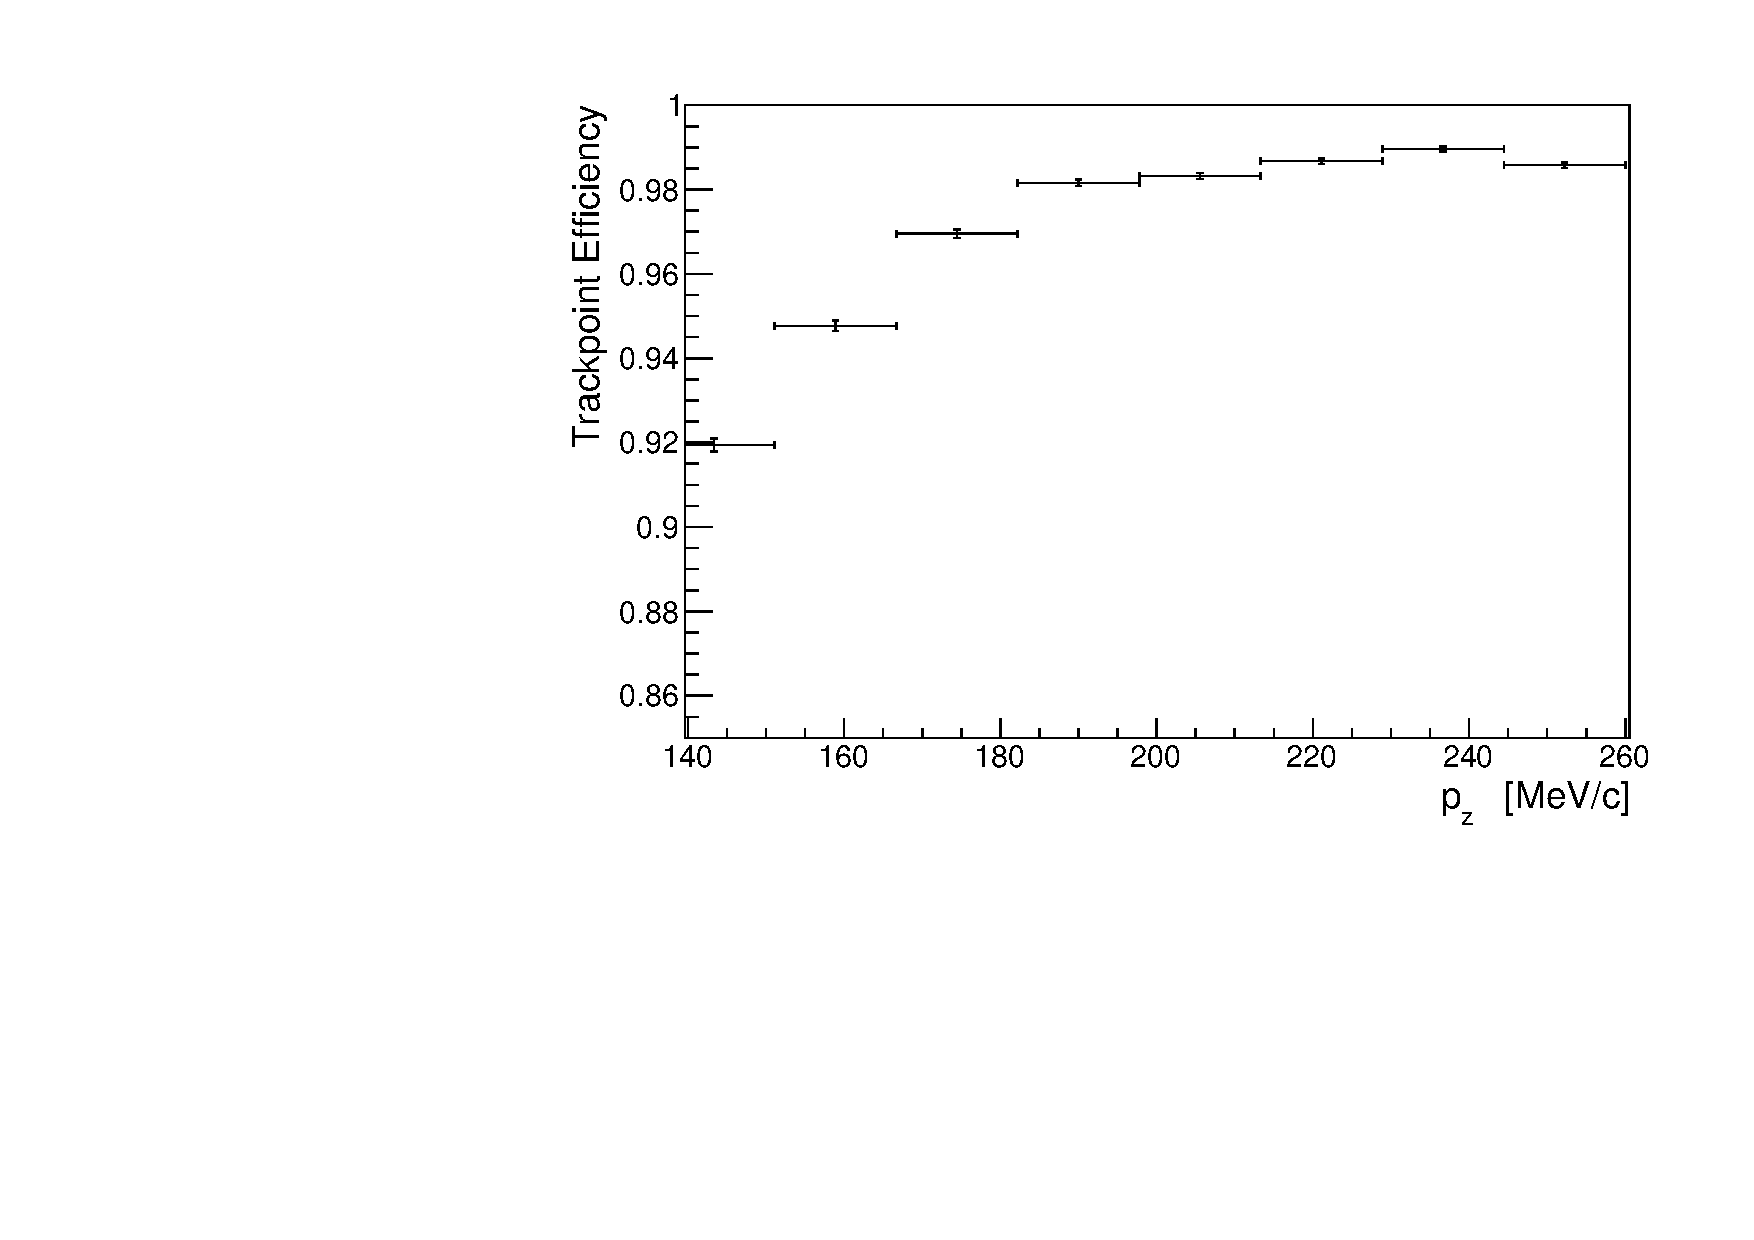
\includegraphics[width=0.45\textwidth, angle=0]{08-Performance/upstream_pz_tp_efficiency.pdf}
    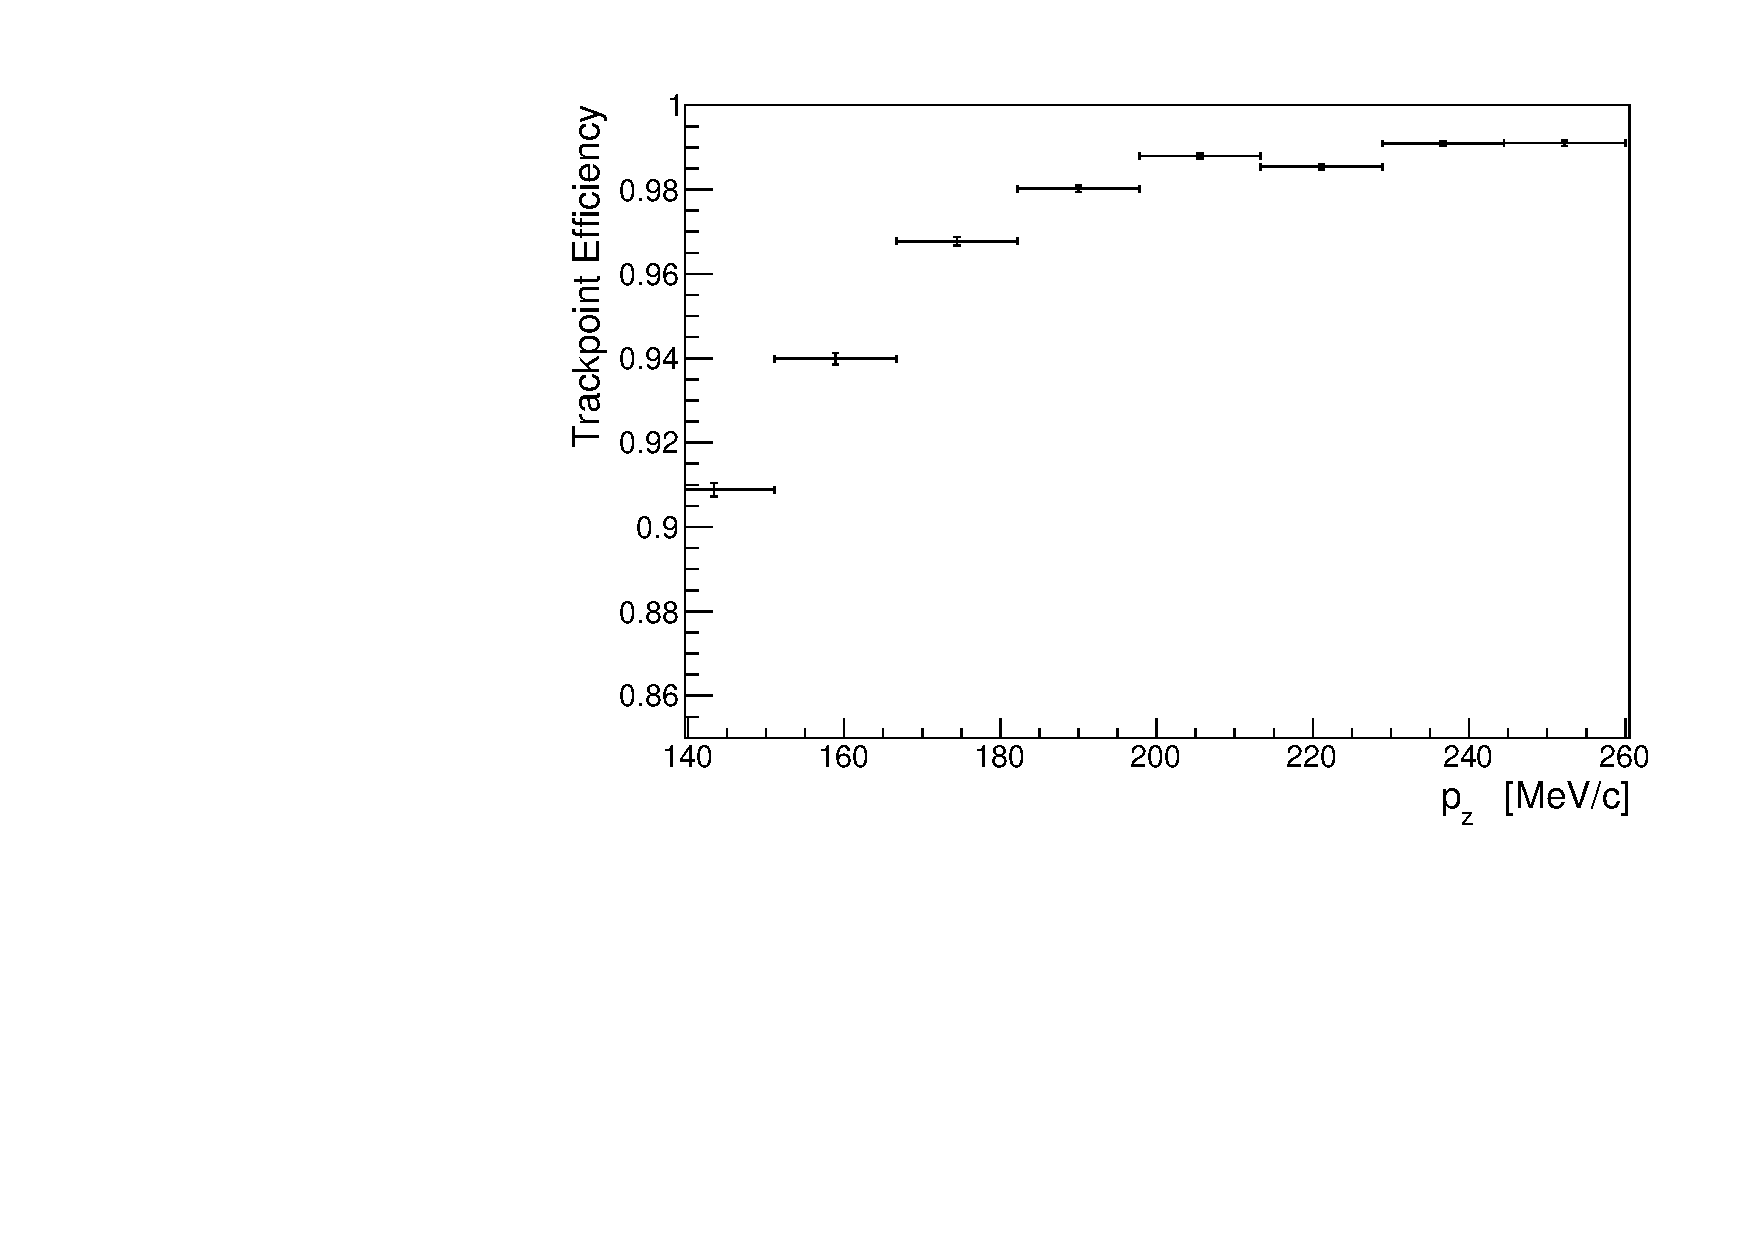
\includegraphics[width=0.45\textwidth, angle=0]{08-Performance/downstream_pz_tp_efficiency.pdf}\\
    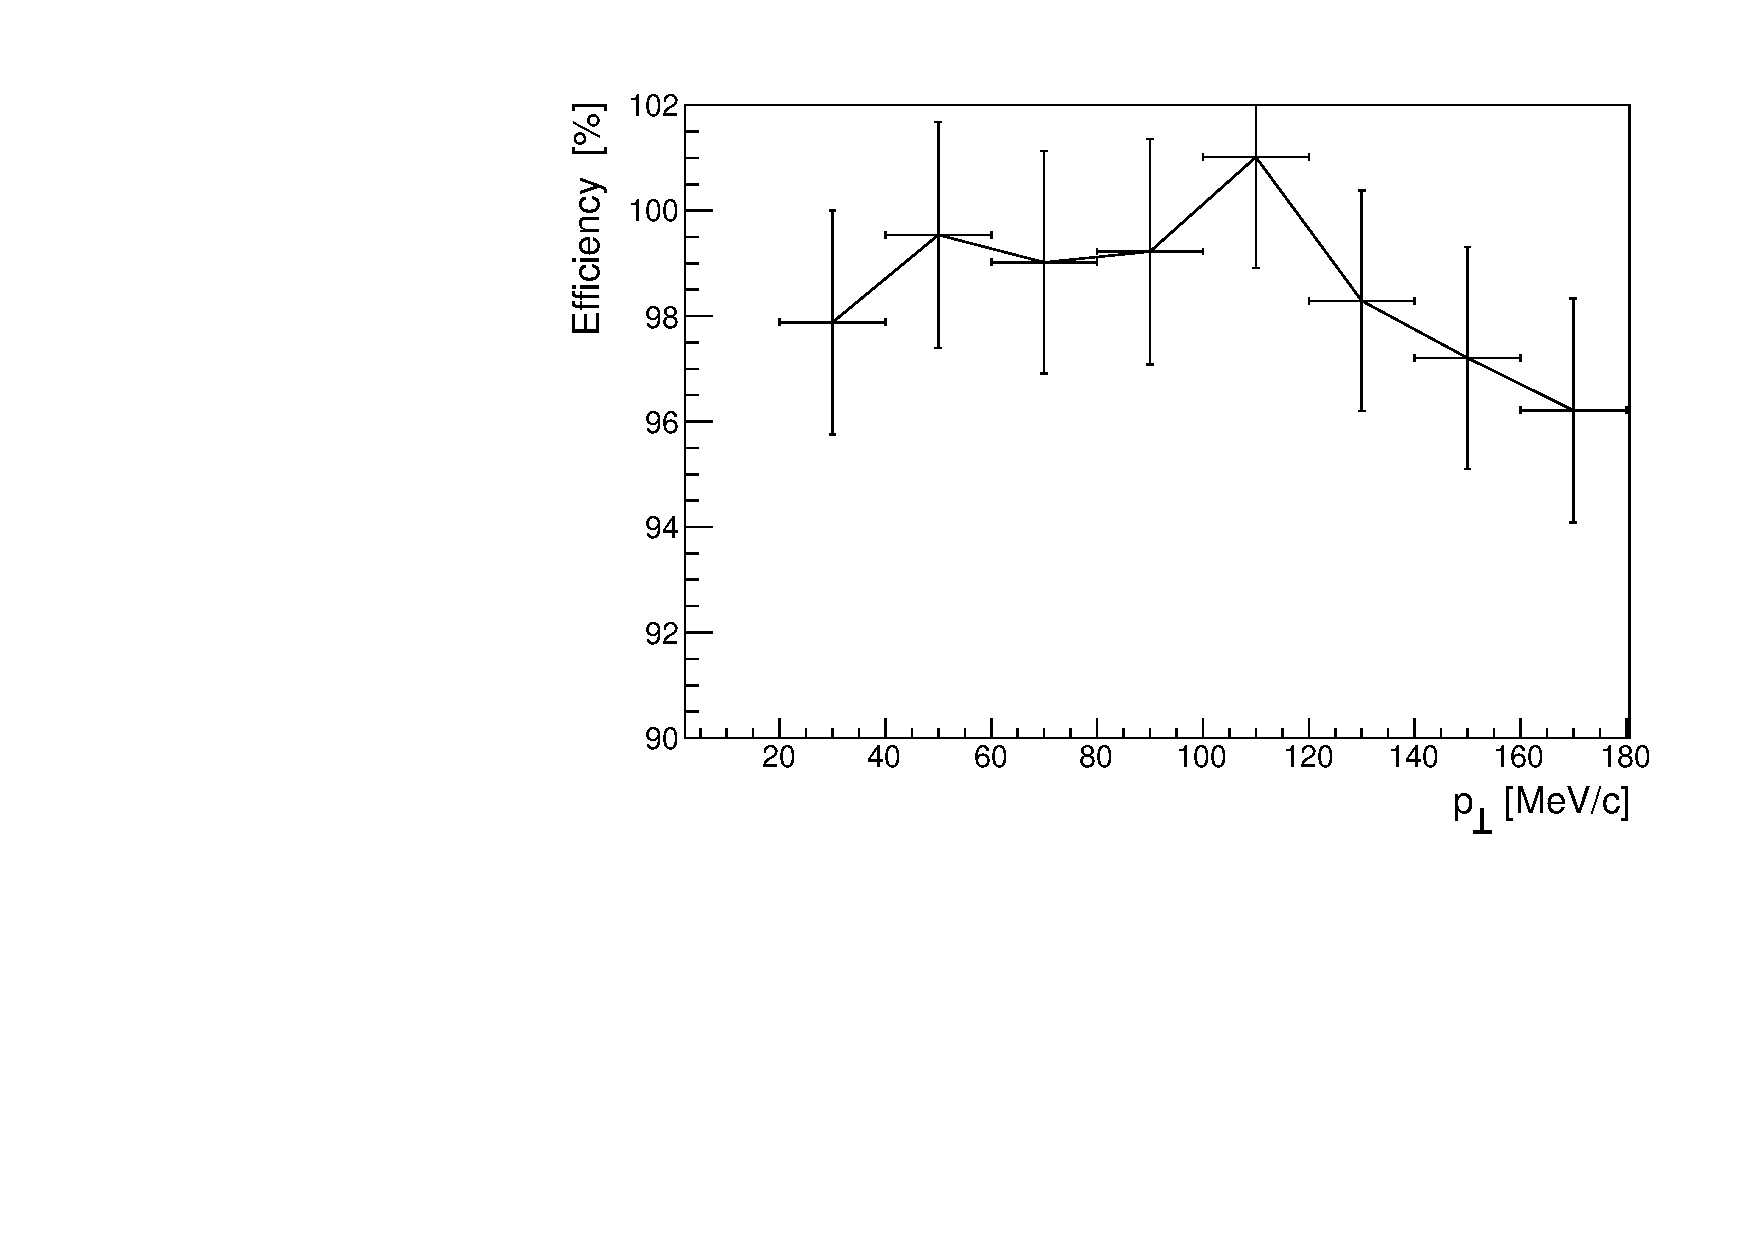
\includegraphics[width=0.45\textwidth, angle=0]{08-Performance/upstream_pt_tp_efficiency.pdf}
    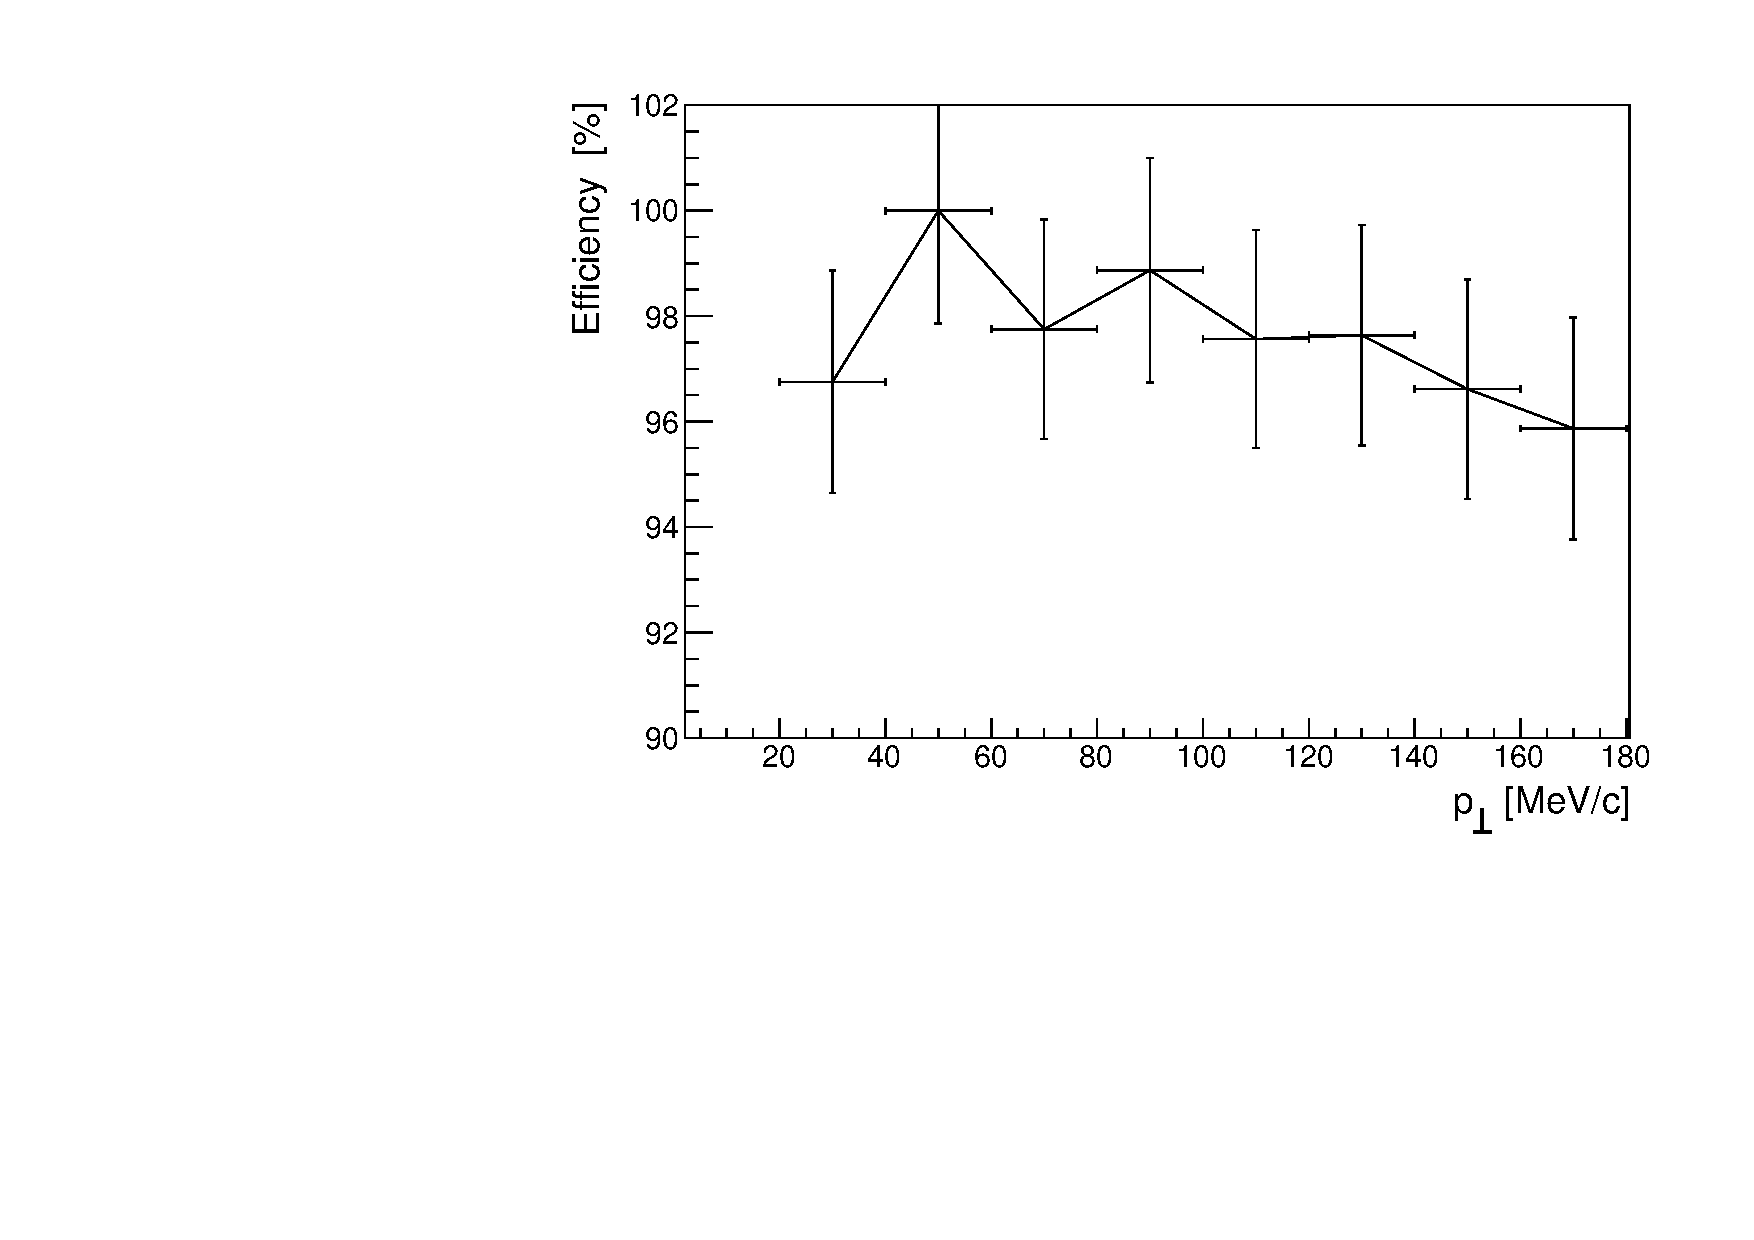
\includegraphics[width=0.45\textwidth, angle=0]{08-Performance/downstream_pt_tp_efficiency.pdf}
    \caption{\label{fig:tp_efficiency} The efficiency of reconstructing trackpoionts in the upstream (left) and downstream (right) trackers as a function of the simulated transverse momentum.}
  \end{figure}


  \subsection{Reconstruction Resolution}
  \label{sec:performance:resolutions}
  
  Position residuals are shown in figures~\ref{fig:XResidKalman} and \ref{fig:YResidKalman}, and the momentum residuals in figures~\ref{fig:PtResidKalman} and \ref{fig:PzResidKalman}.  The position reconstruction can be seen to agree with the Monte Carlo truth to high precision in both the upstream and downstream trackers. The momentum residuals currently display some systematic effect which is due to a known issue with the energy loss determination and is currently under study.
  
  In order to produce these plots, a requirement that there was a cluster within the reference plane was applied. Due to the effects of Multiple Coulomb Scattering, on rare occaisons a single hard scatter can cause pattern recognition to miss a single spacepoint at the reference plane, hence creating a tail that will adversely affect the distrubtions. As we are concerned with the resolution following a successful pattern recognition stage, these events were removed.
  
  The position residuals are consistent with the expected measurement resolutions for a combined fit and the absolute spread is very close to the width of a channel (1.497mm). The transverse momentum resolution is consitent accross the range of the sensitive phase space at $\sim$1~MeV/c in both trackers. The longitudinal momentum, an intrinsically more difficult measurement for the tracker, still retains an acceptable spread of $\sim3$~MeV/c in both trackers. There is however a systematic offset present in the distributions, 1.5~MeV/c in the upstream tracker, and 3.5~MeV/c in the downstream, and the distributions have more pronounced tails than in the transverse cases. These offsets require further investigation.
  
  Trends in transverse and longitudinal momentum resolution as a function of transverse momentum are shown in figures~\ref{fig:PtPtResolKalman} and \ref{fig:PtPzResolKalman}. A consistently uniform distribution is found in the transverse momentum as exected, with the predominant issue found in the longitudinal reconstruction of low-$P_t$ tracks. This effect, when coupled with variations in efficiency will yield some systematic concerns in the reconstruction of statistical quantities such as emittance. Studies of these systematic biases are currently underway.

  \begin{figure}[p]
    \begin{center}
      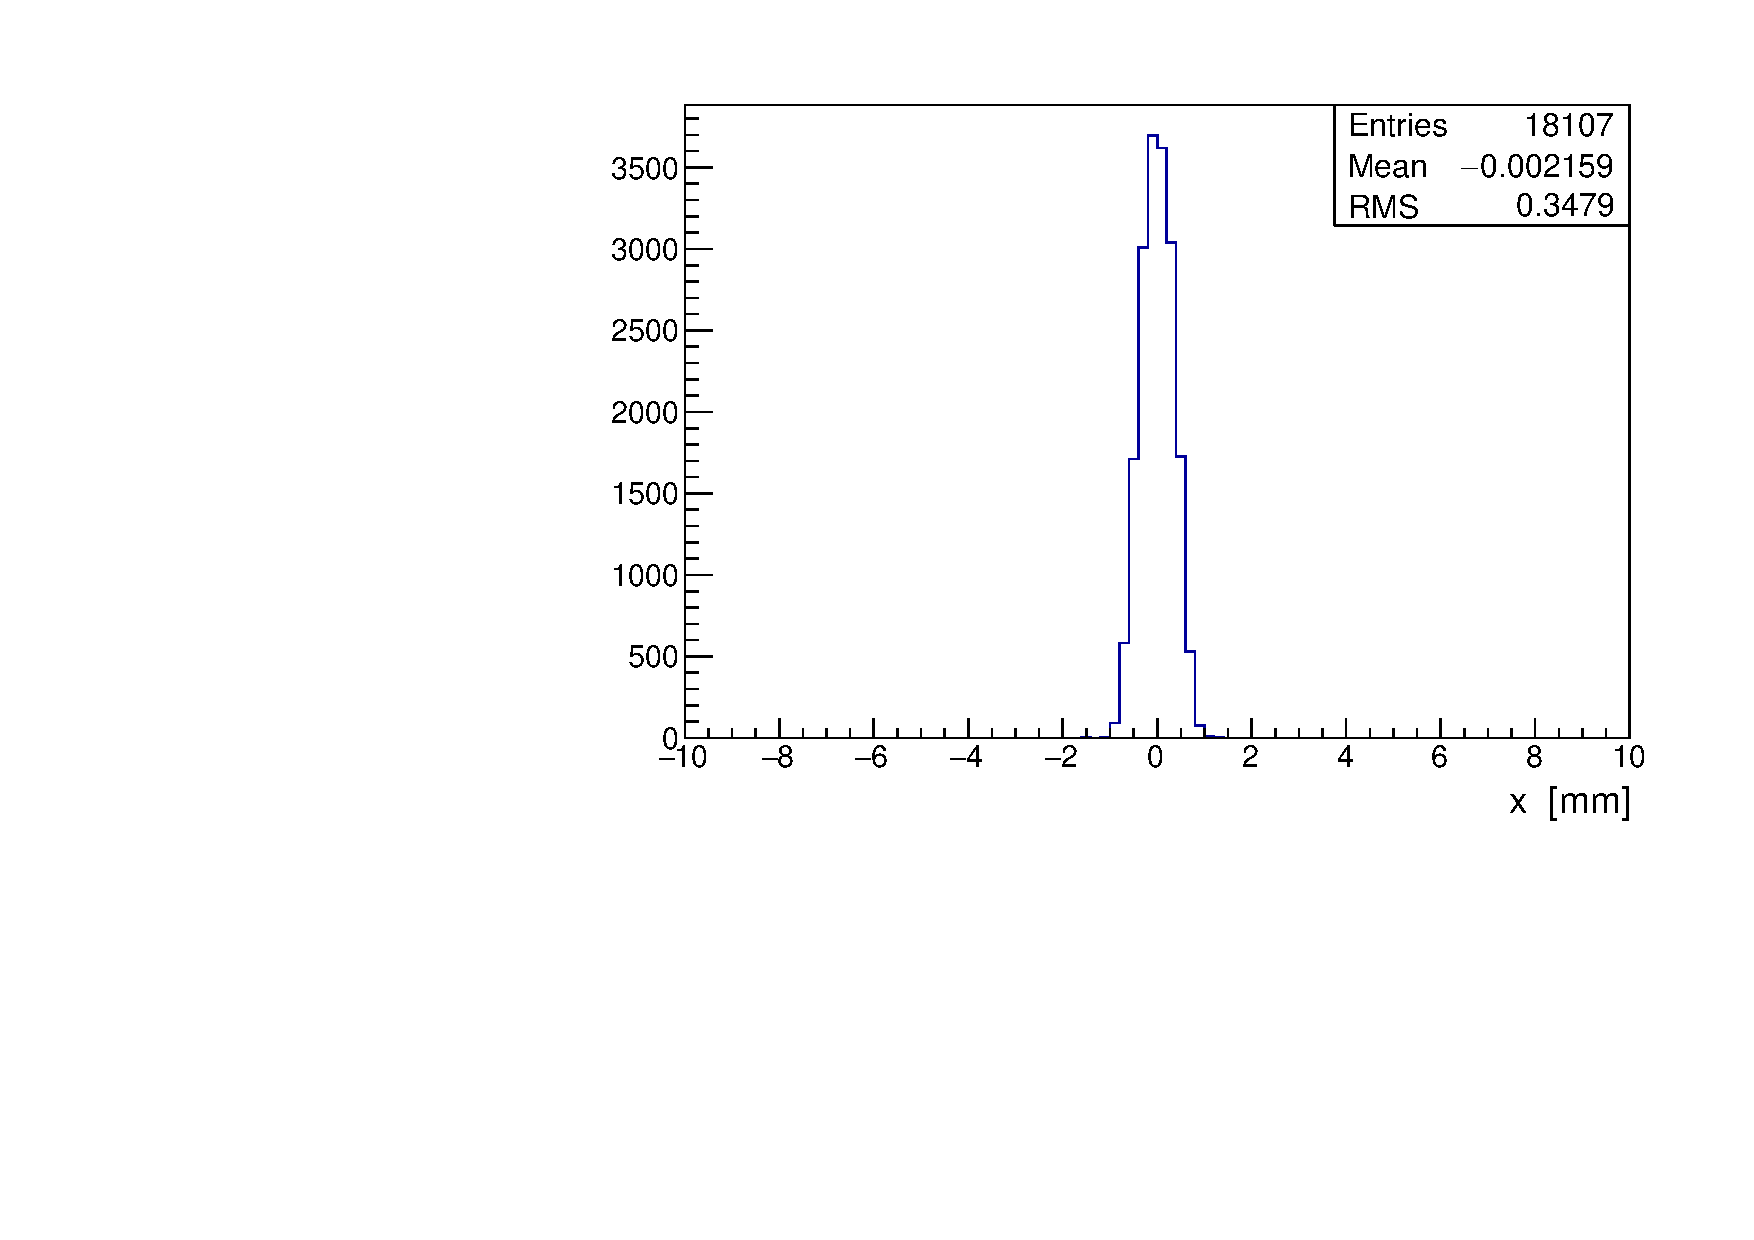
\includegraphics[width=0.49\textwidth, angle=0]{08-Performance/upstream_x_residudal.pdf}
      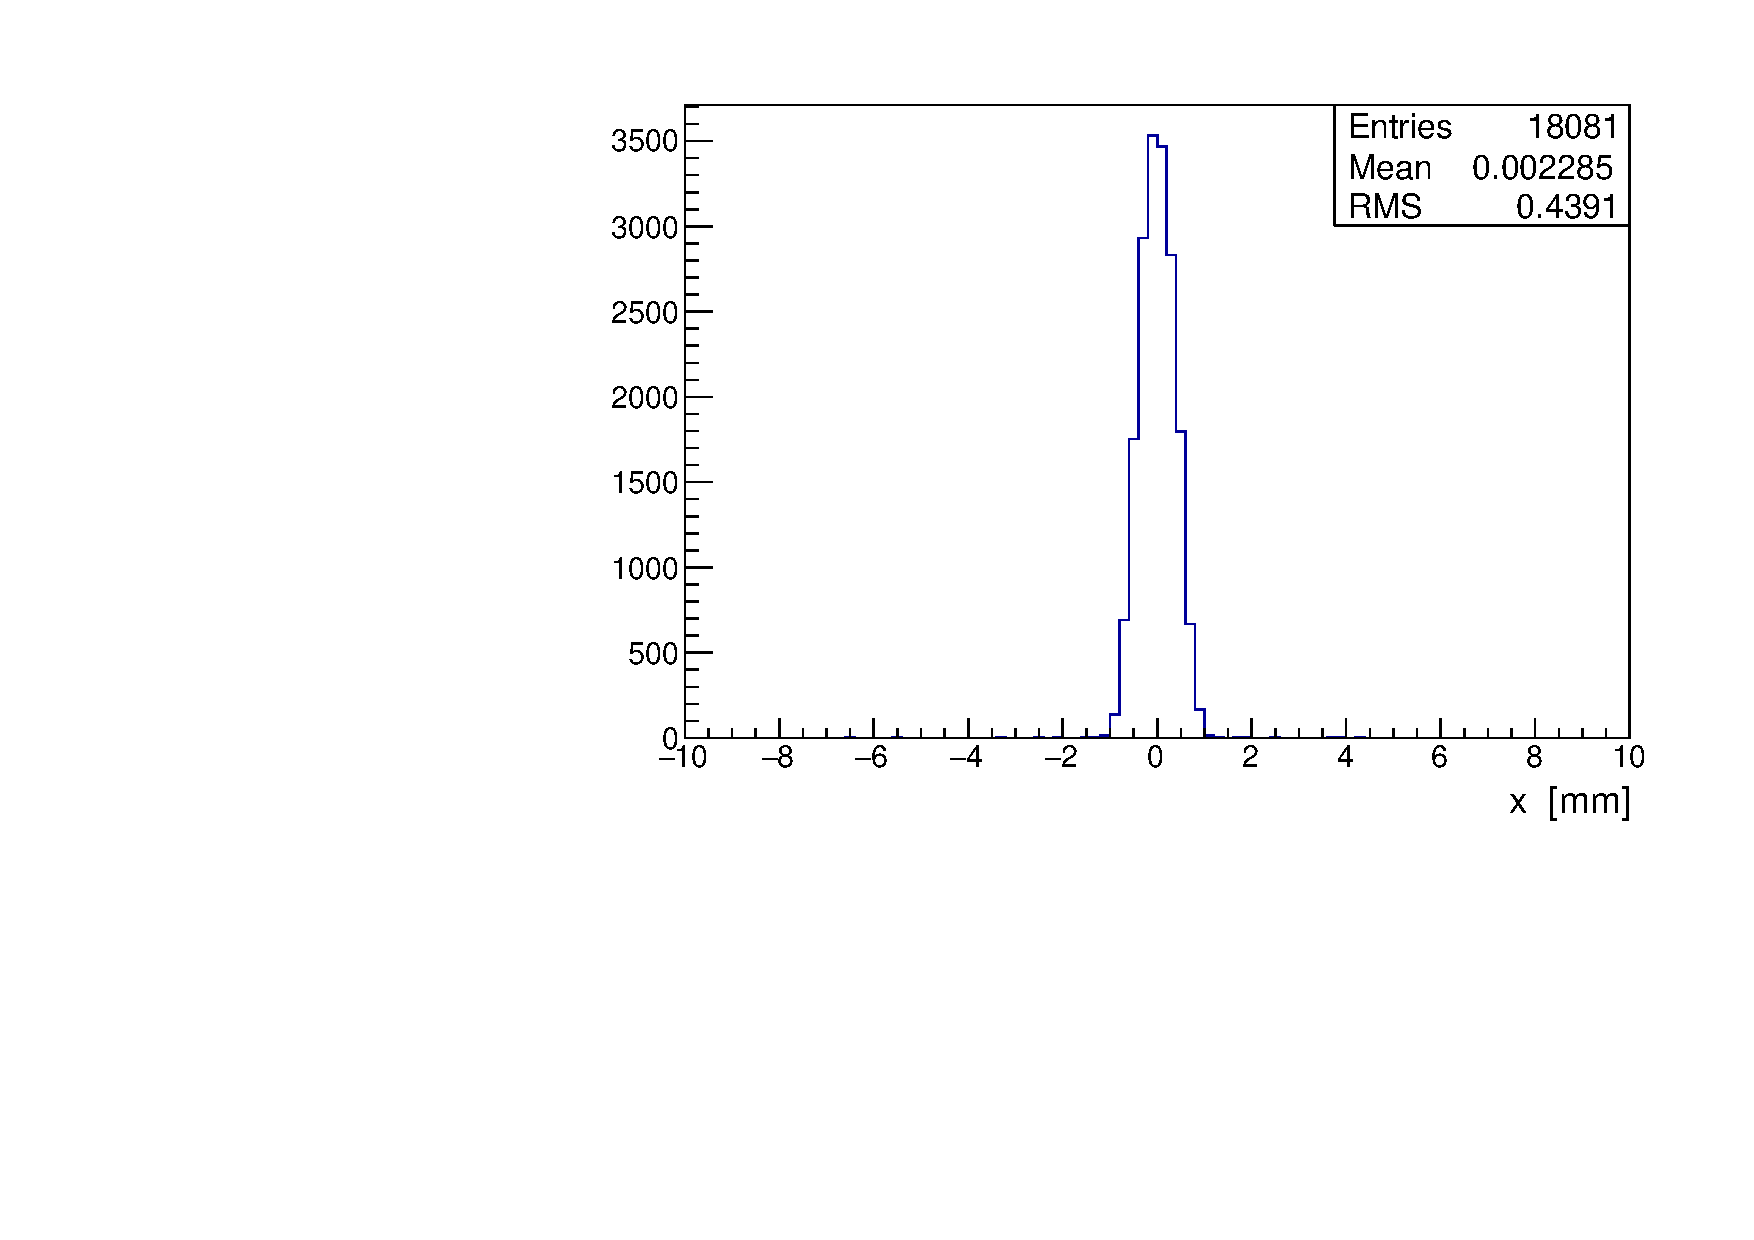
\includegraphics[width=0.49\textwidth, angle=0]{08-Performance/downstream_x_residudal.pdf}
      \caption{\label{fig:XResidKalman} The $x$ residuals of the upstream (left) and downstream (right) trackers for a 6~mm 4D emittance, and 200~MeV/c momentum beam.}
    \end{center}
  \end{figure}
  
    \begin{figure}[p]
    \begin{center}
      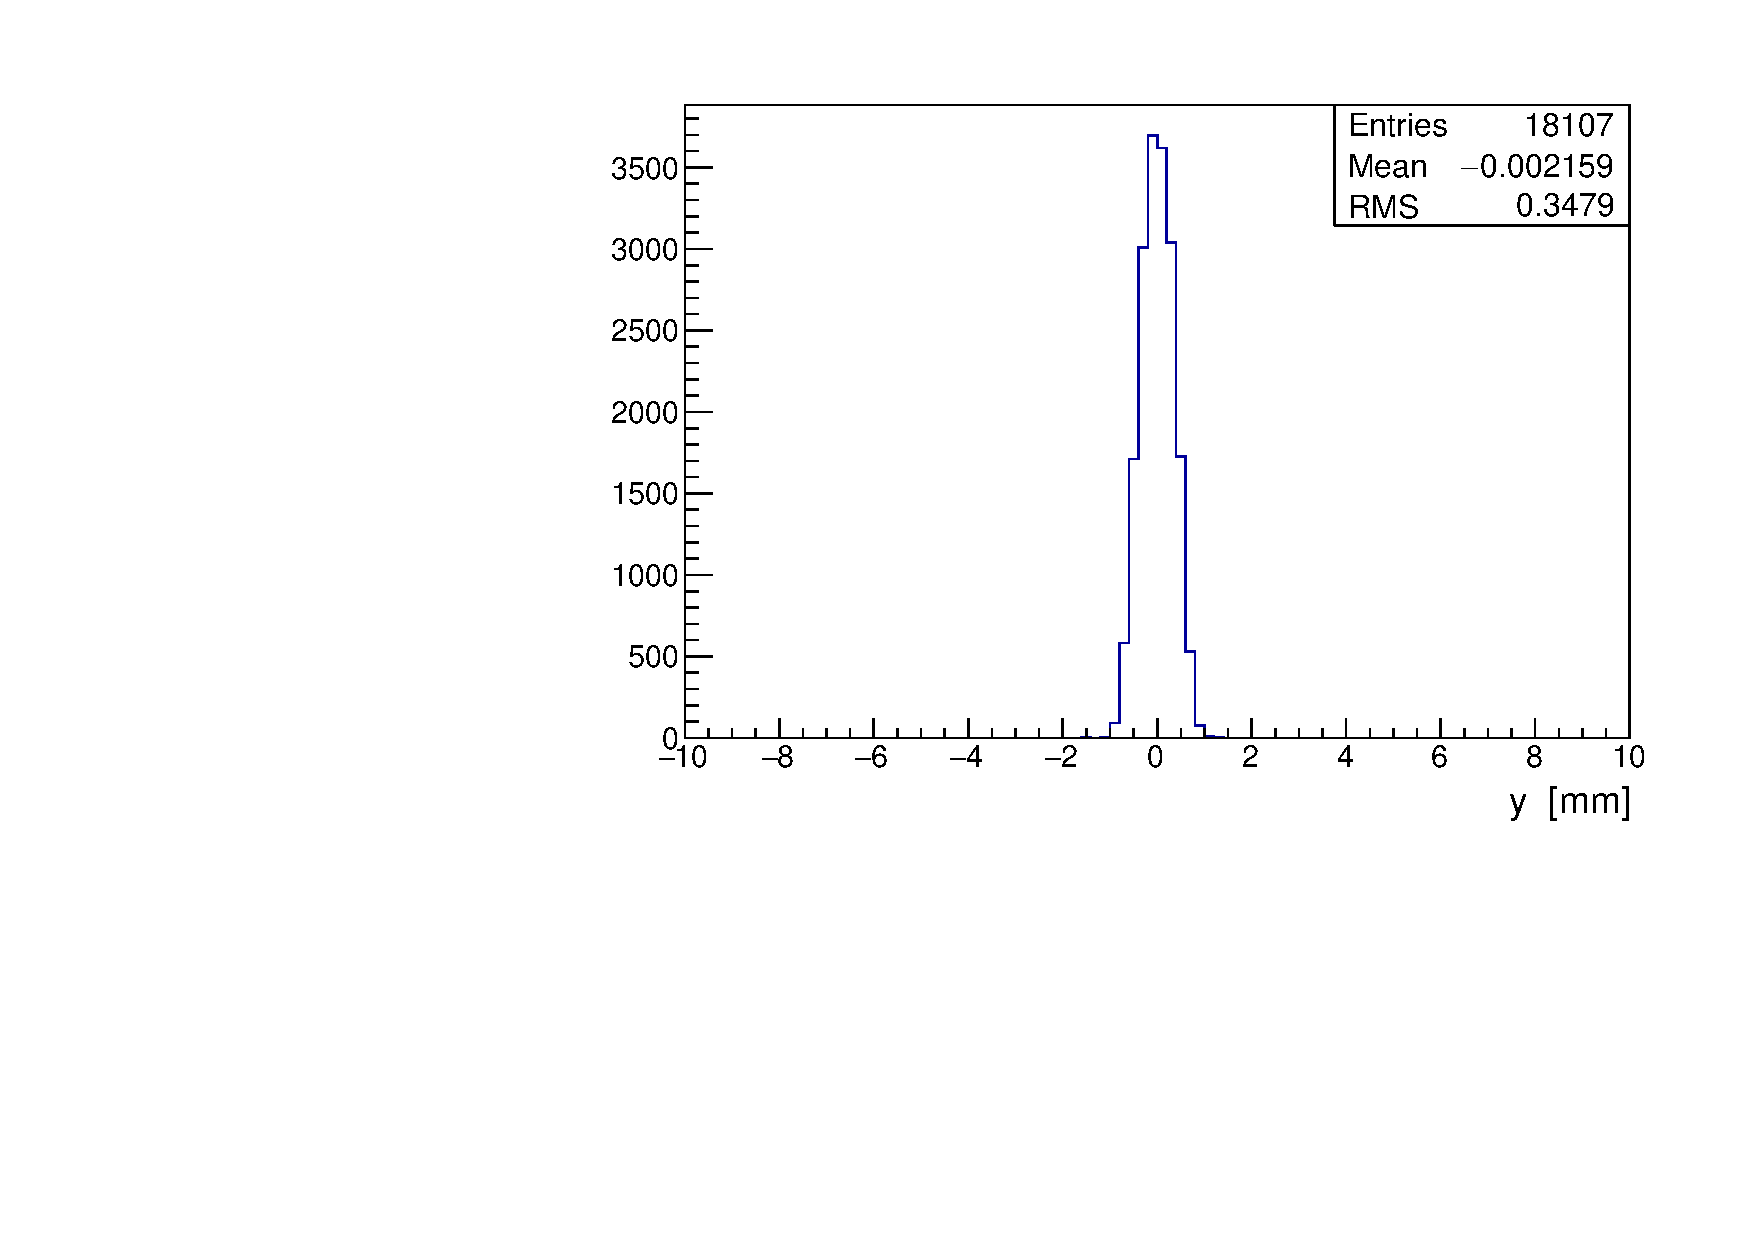
\includegraphics[width=0.49\textwidth, angle=0]{08-Performance/upstream_y_residudal.pdf}
      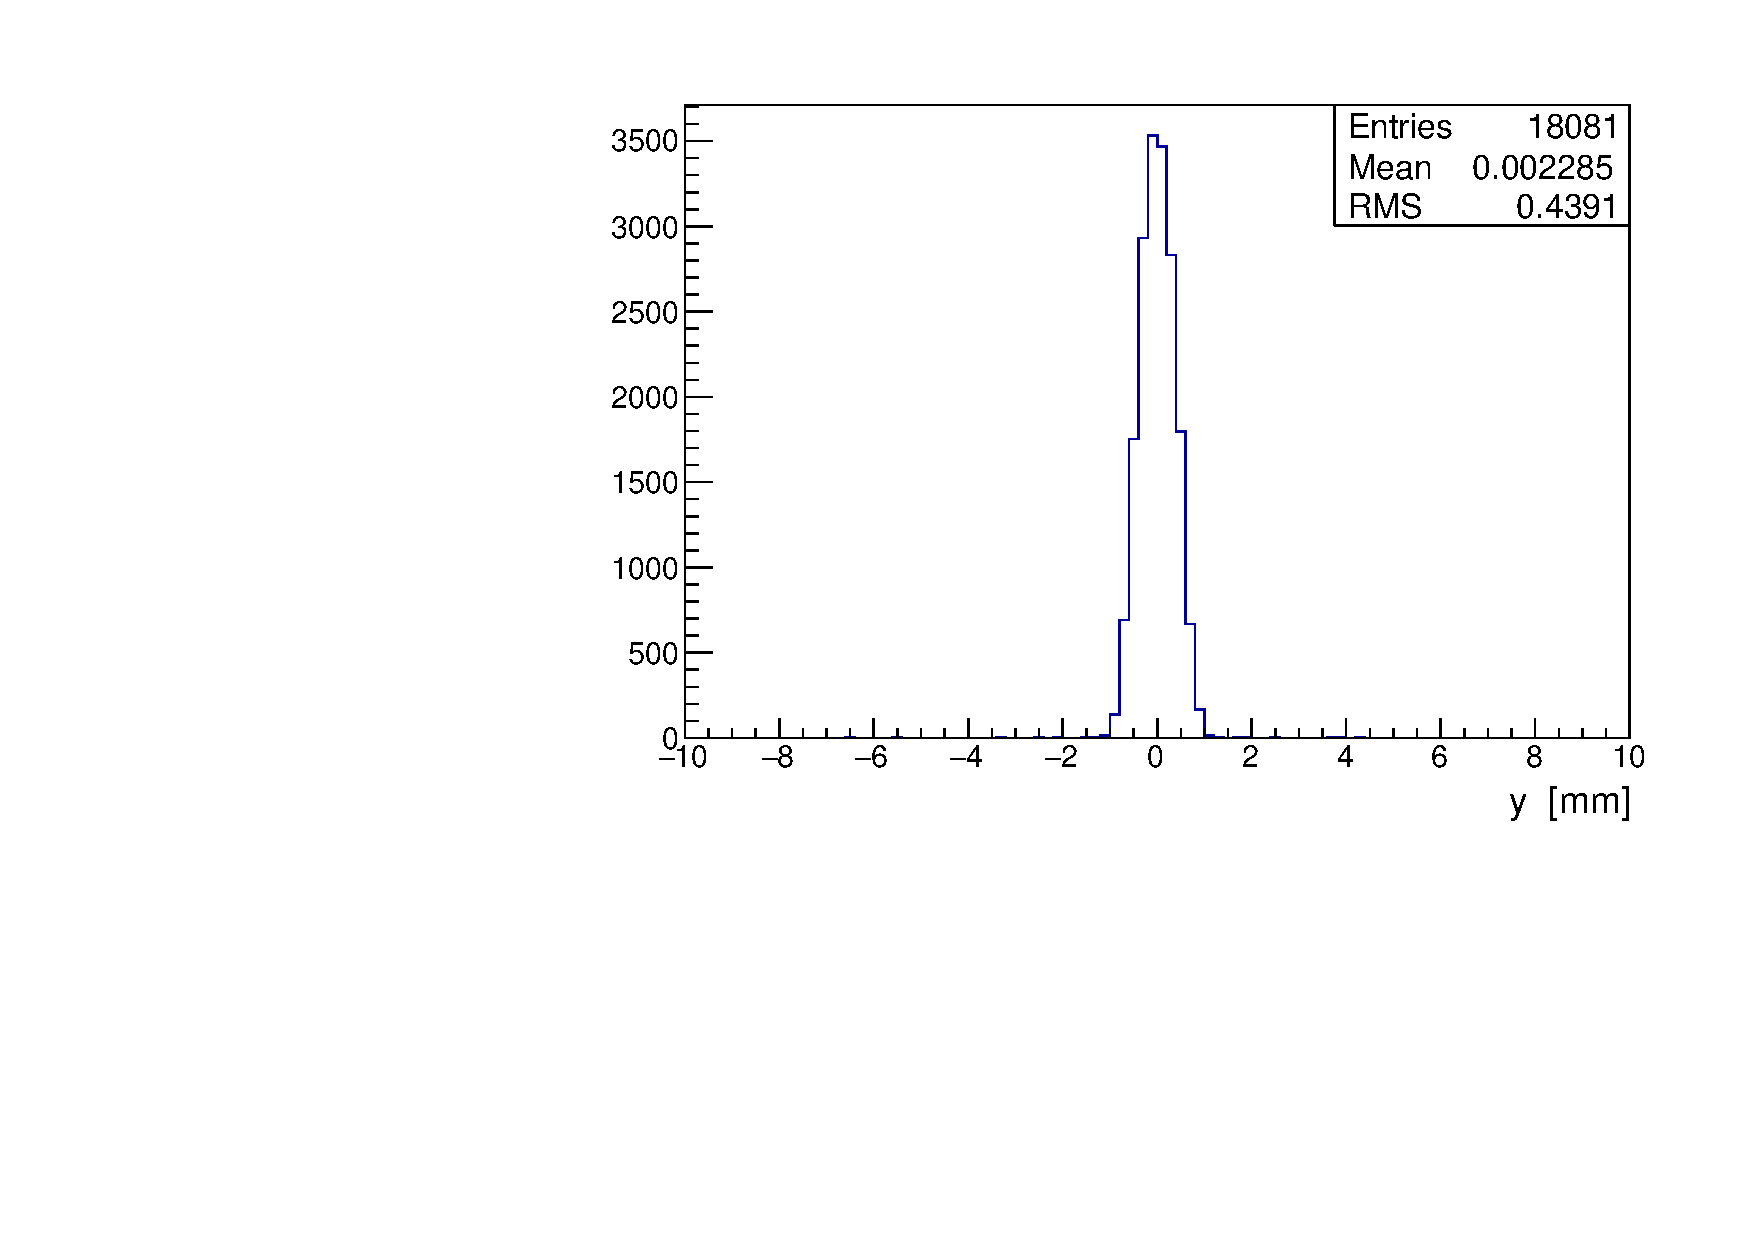
\includegraphics[width=0.49\textwidth, angle=0]{08-Performance/downstream_y_residudal.pdf}
      \caption{\label{fig:YResidKalman} The $y$ residuals of the upstream (left) and downstream (right) trackers for a 6~mm 4D emittance, and 200~MeV/c momentum beam.}
    \end{center}
  \end{figure}
  
  
  \begin{figure}[p]
    \begin{center}
      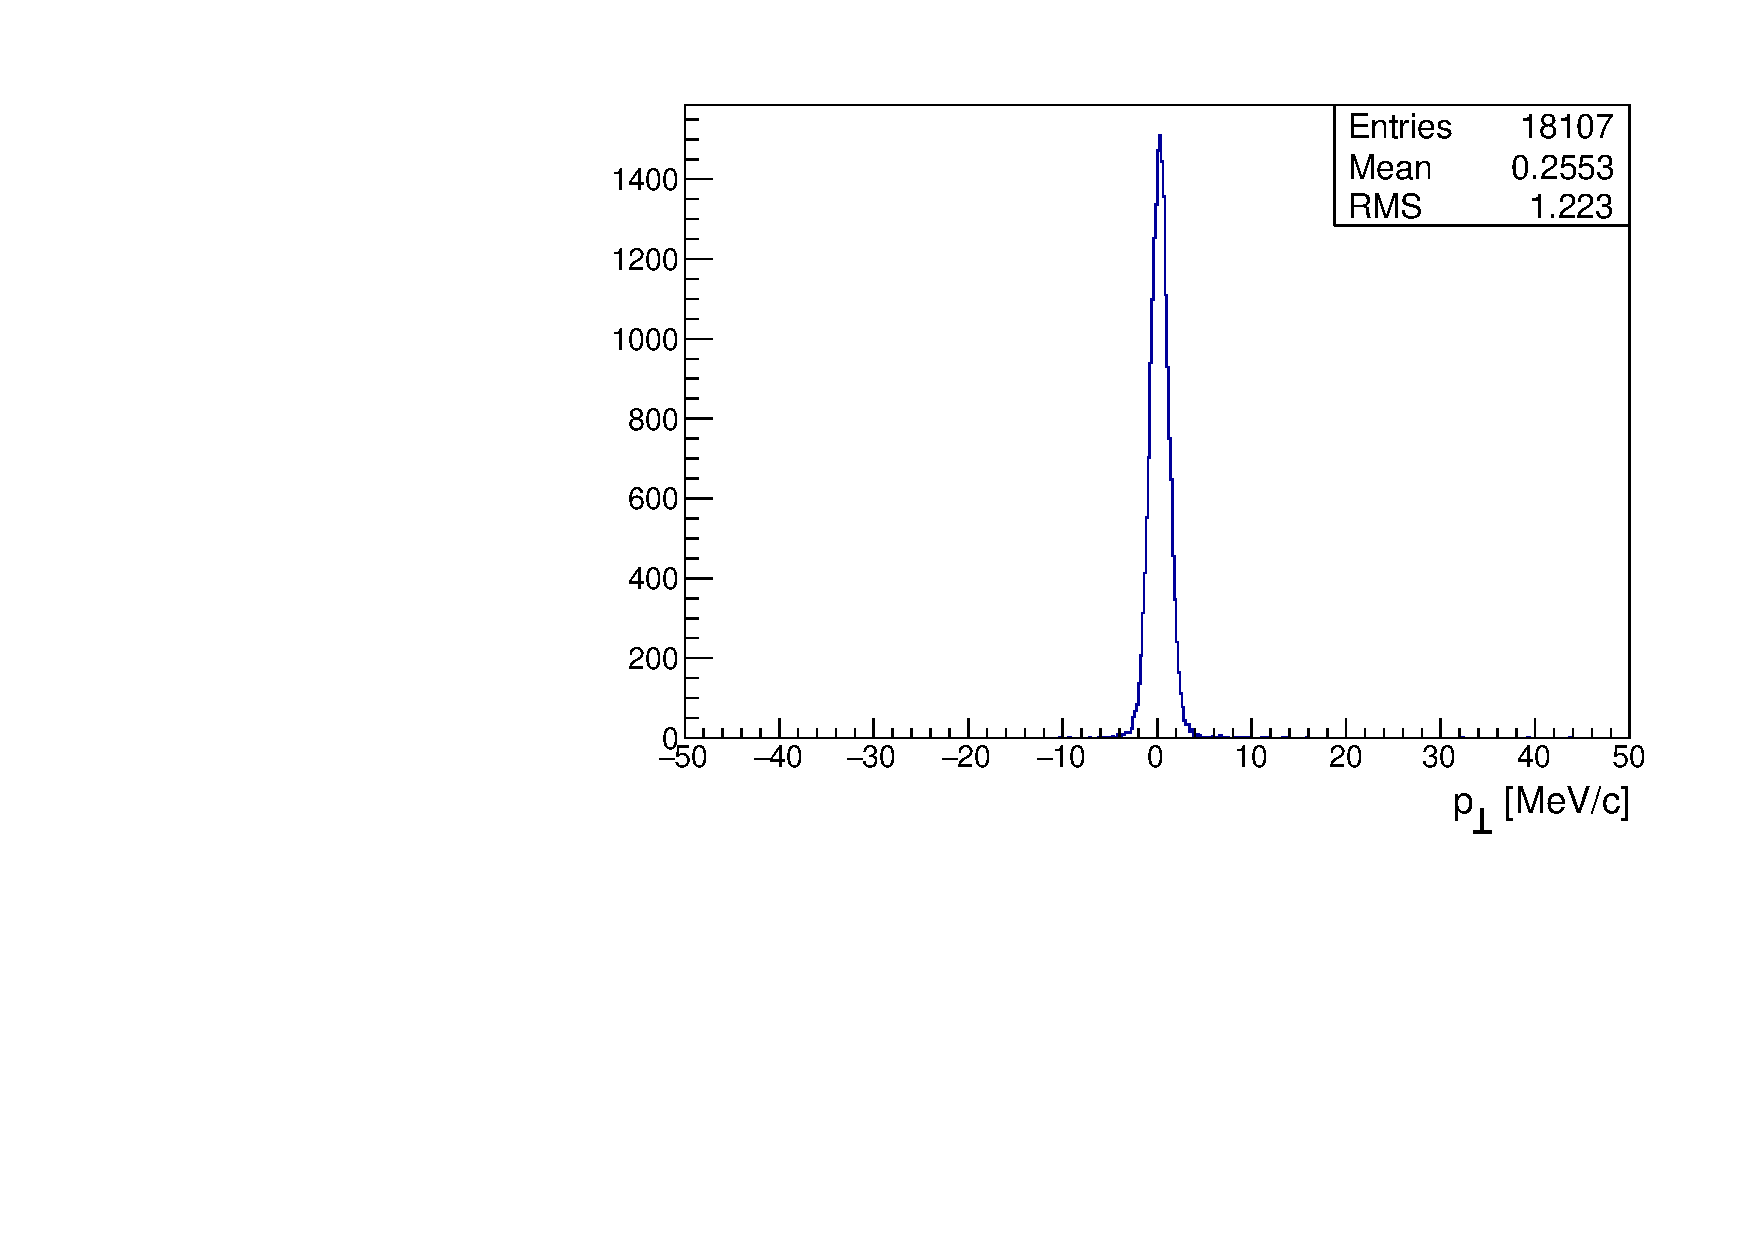
\includegraphics[width=0.49\textwidth, angle=0]{08-Performance/upstream_pt_residudal.pdf}
      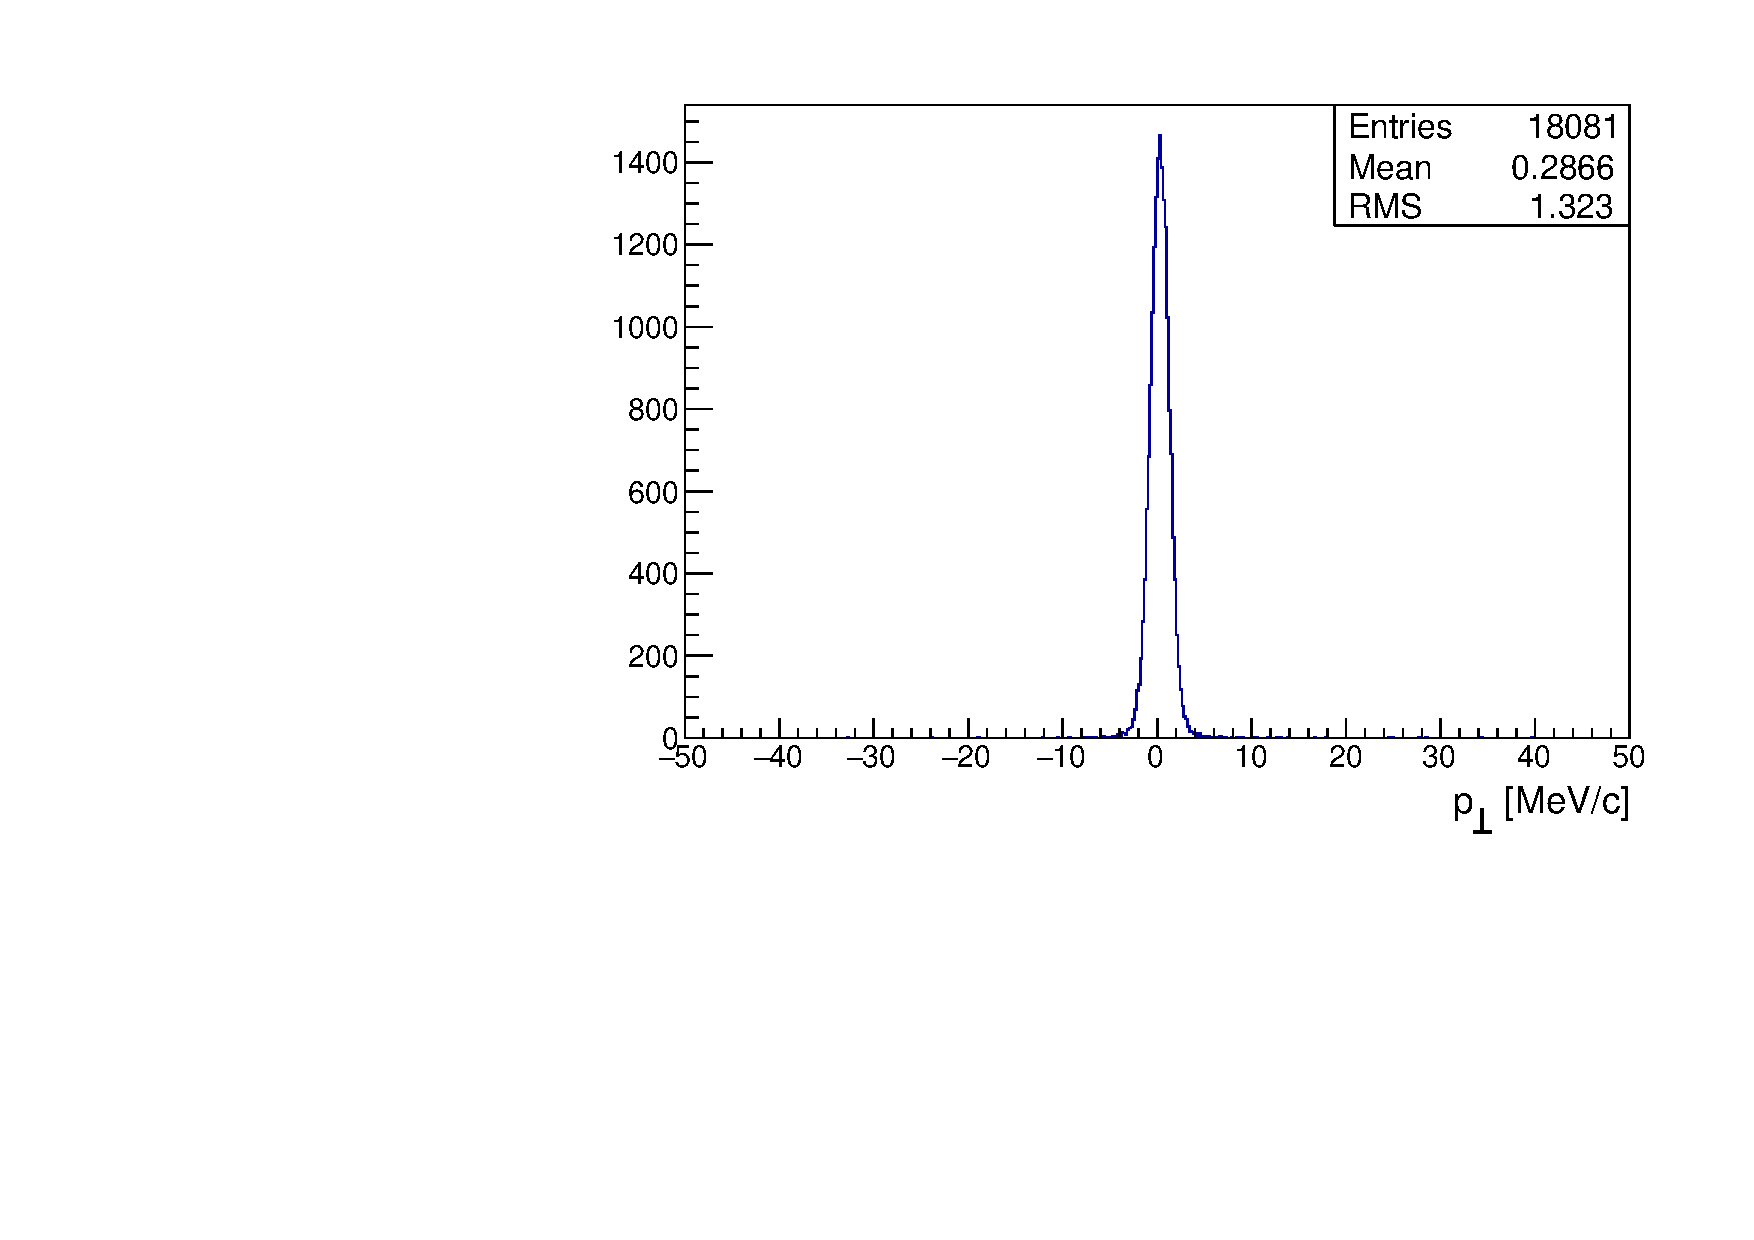
\includegraphics[width=0.49\textwidth, angle=0]{08-Performance/downstream_pt_residudal.pdf}
      \caption{\label{fig:PtResidKalman} The $p_{\perp}$ residuals of the upstream (left) and downstream (right).}
    \end{center}
  \end{figure}
  
   \begin{figure}[p]
    \begin{center}
      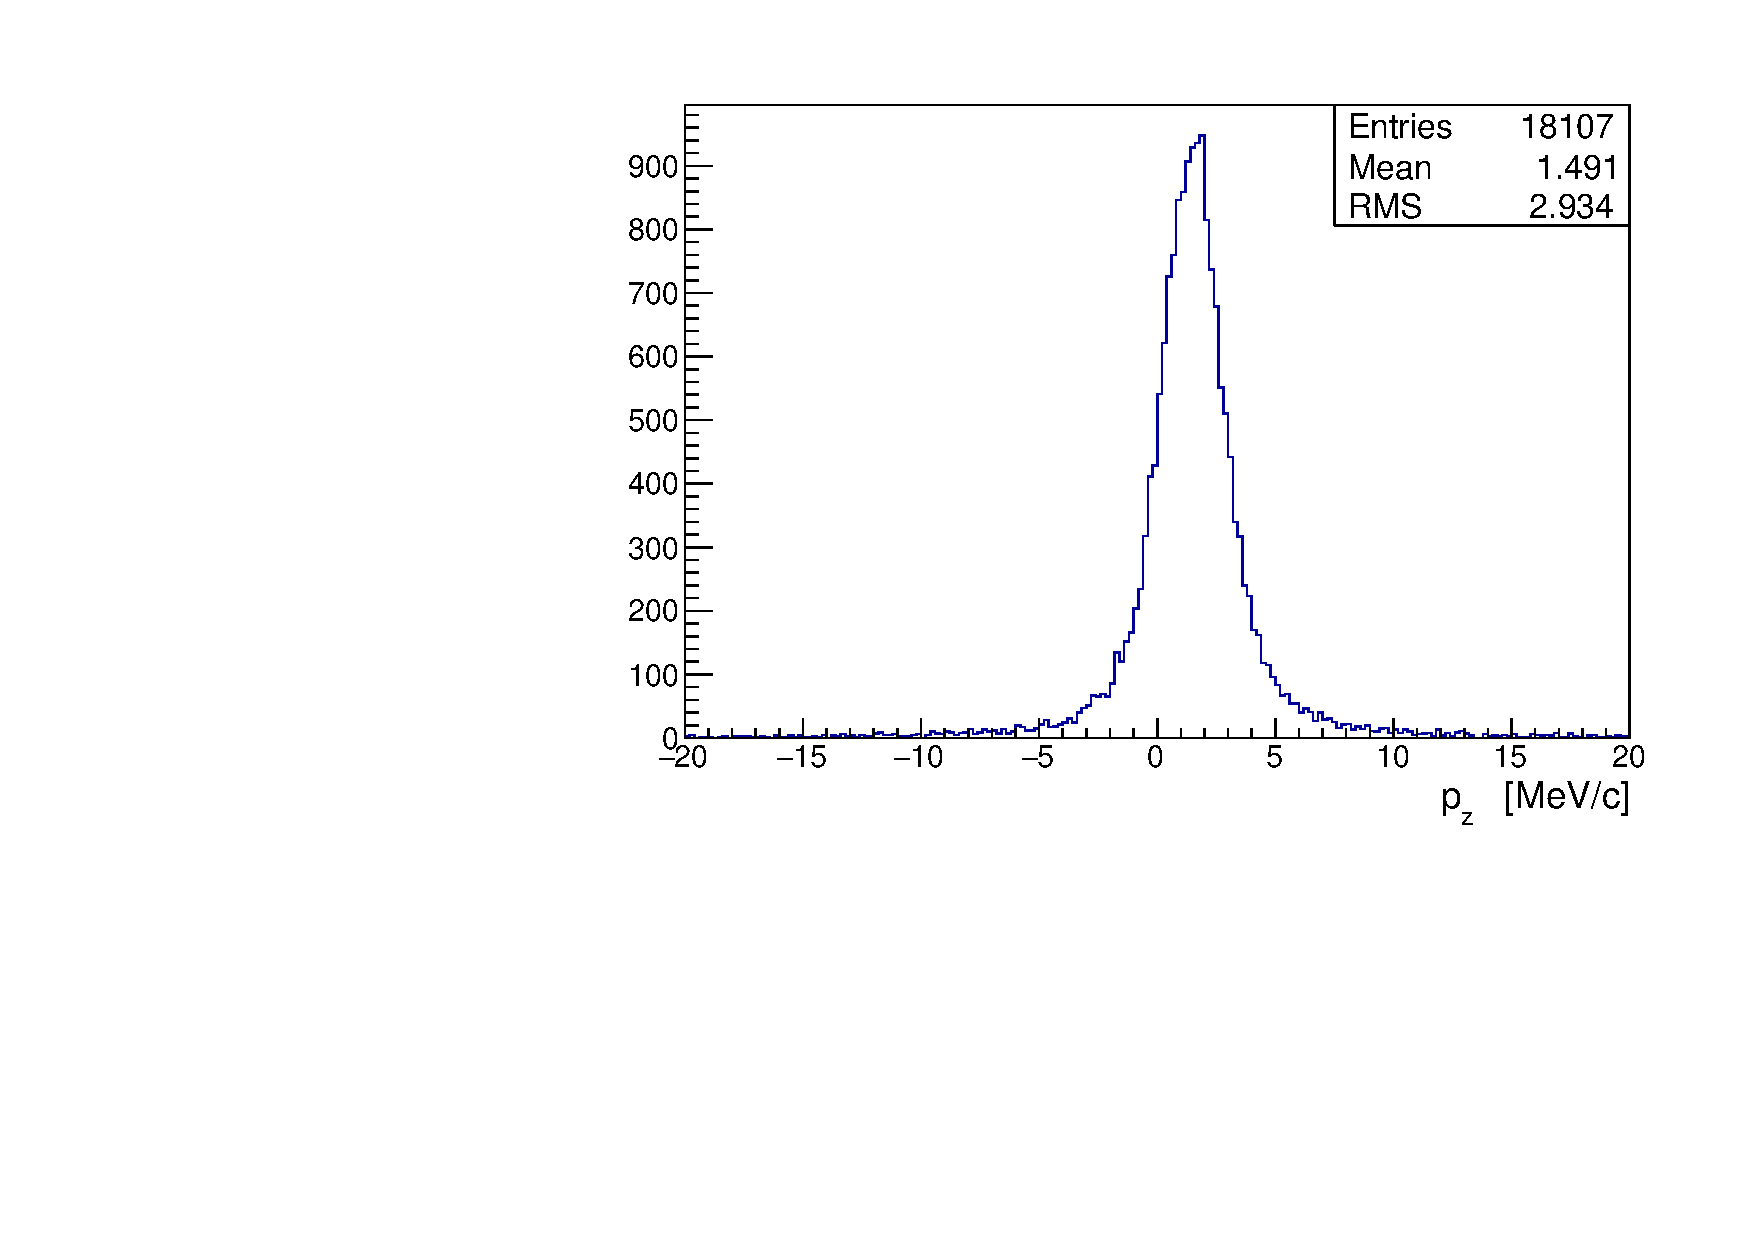
\includegraphics[width=0.49\textwidth, angle=0]{08-Performance/upstream_pz_residudal.pdf}
      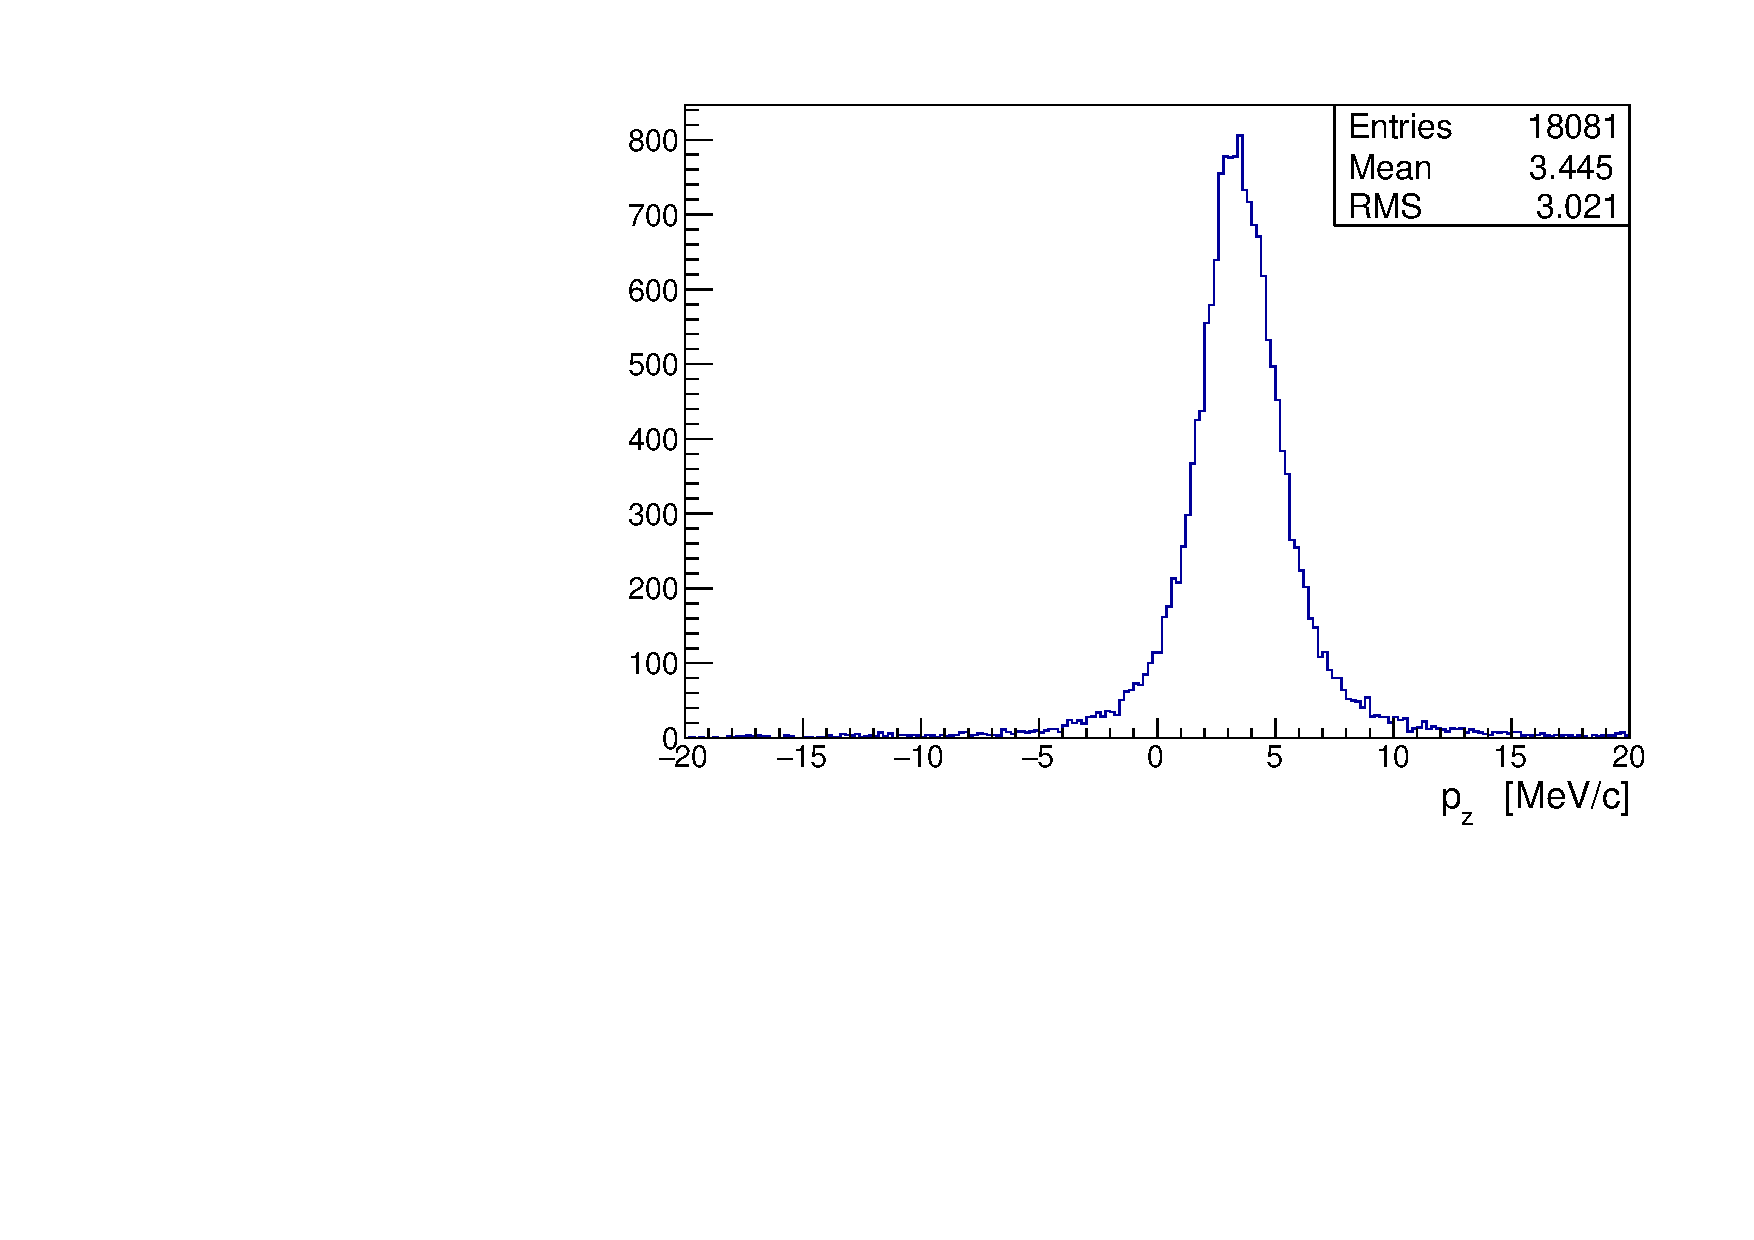
\includegraphics[width=0.49\textwidth, angle=0]{08-Performance/downstream_pz_residudal.pdf}
      \caption{\label{fig:PzResidKalman} The $p_z$ residuals of the upstream (left) and downstream (right) trackers for a 6~mm 4D emittance, and 200~MeV/c momentum beam.}
    \end{center}
  \end{figure}
  
  \begin{figure}[p]
   \begin{center}
     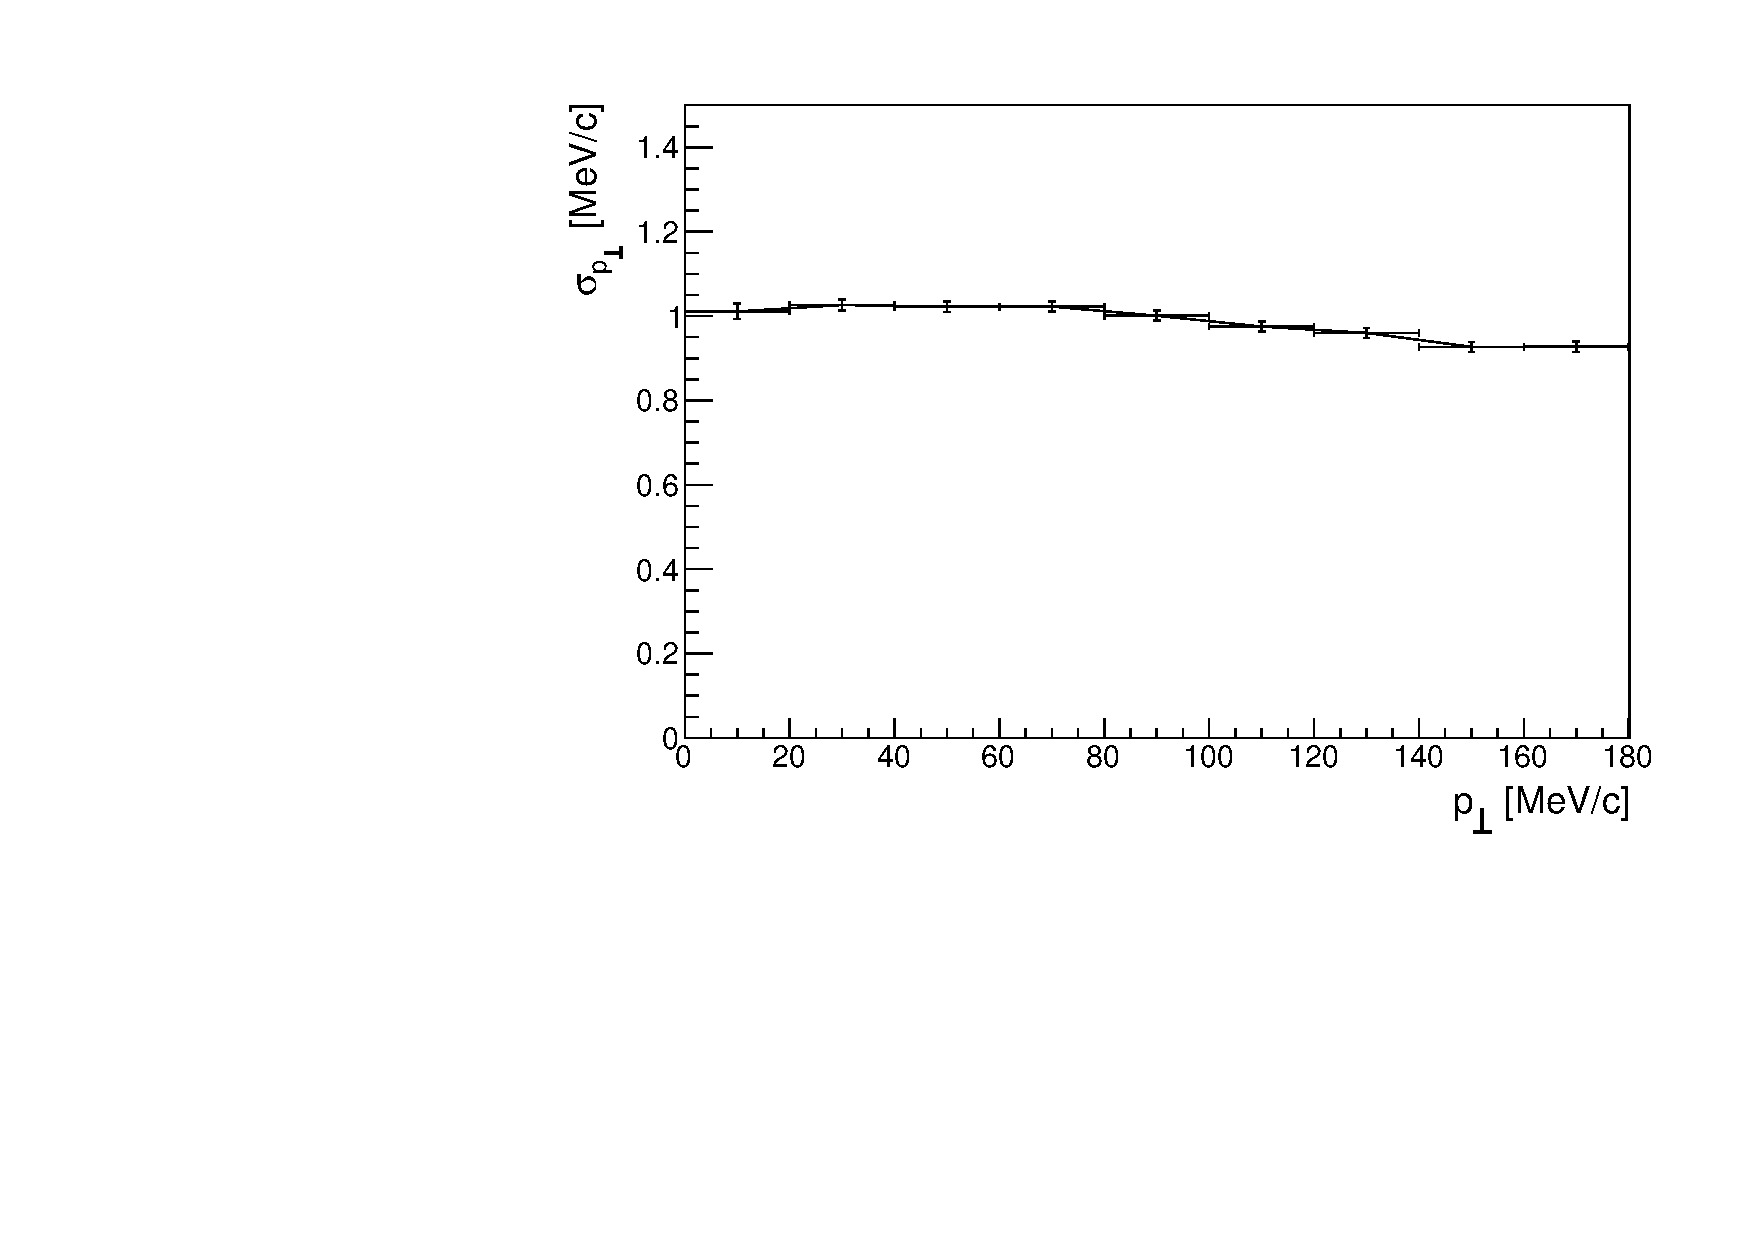
\includegraphics[width=0.49\textwidth, angle=0]{08-Performance/upstream_pt_resolution_pt.pdf}
     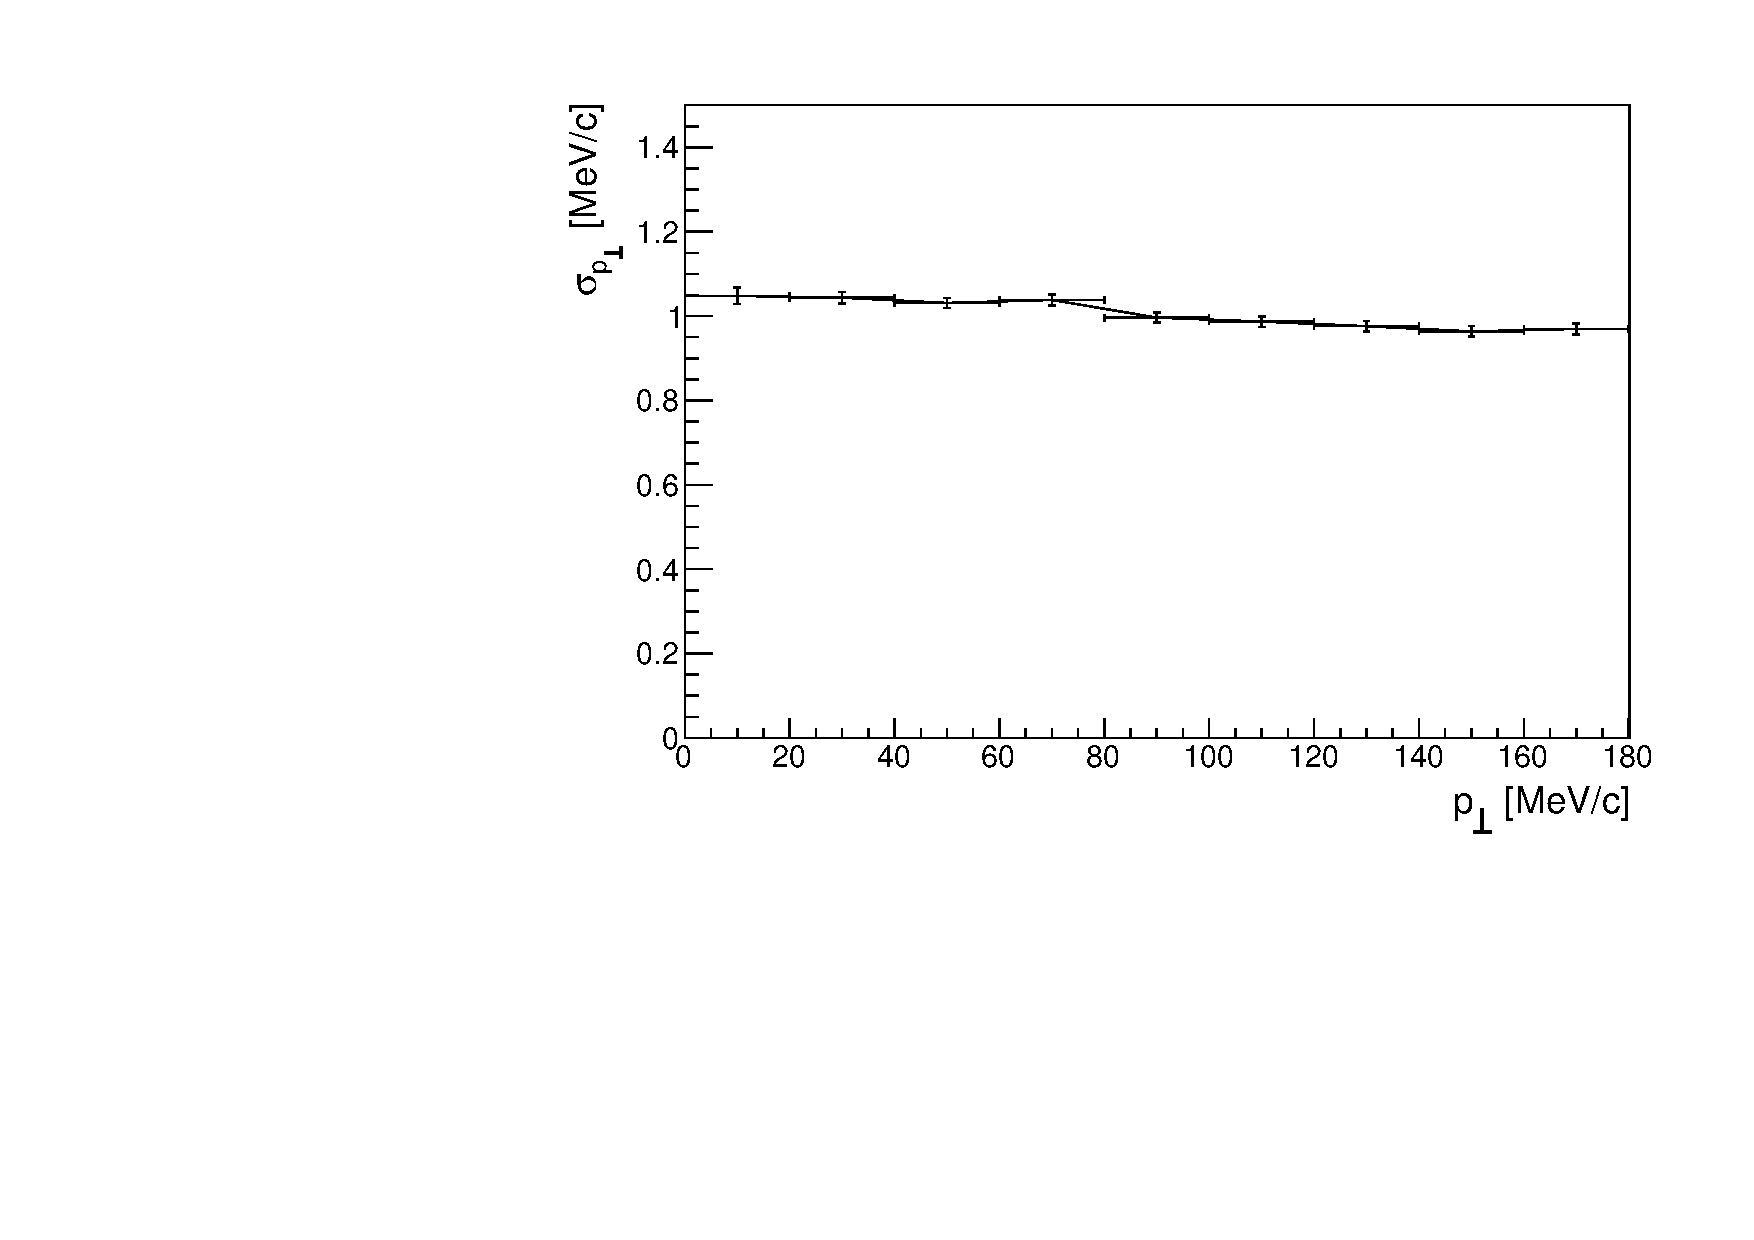
\includegraphics[width=0.49\textwidth, angle=0]{08-Performance/downstream_pt_resolution_pt.pdf}
     \caption{\label{fig:PtPtResolKalman} The $p_{\perp}$ resolution vs the $p_{\perp}$ of the upstream (left) and downstream (right).}
   \end{center}
  \end{figure}
  
  \begin{figure}[p]
   \begin{center}
     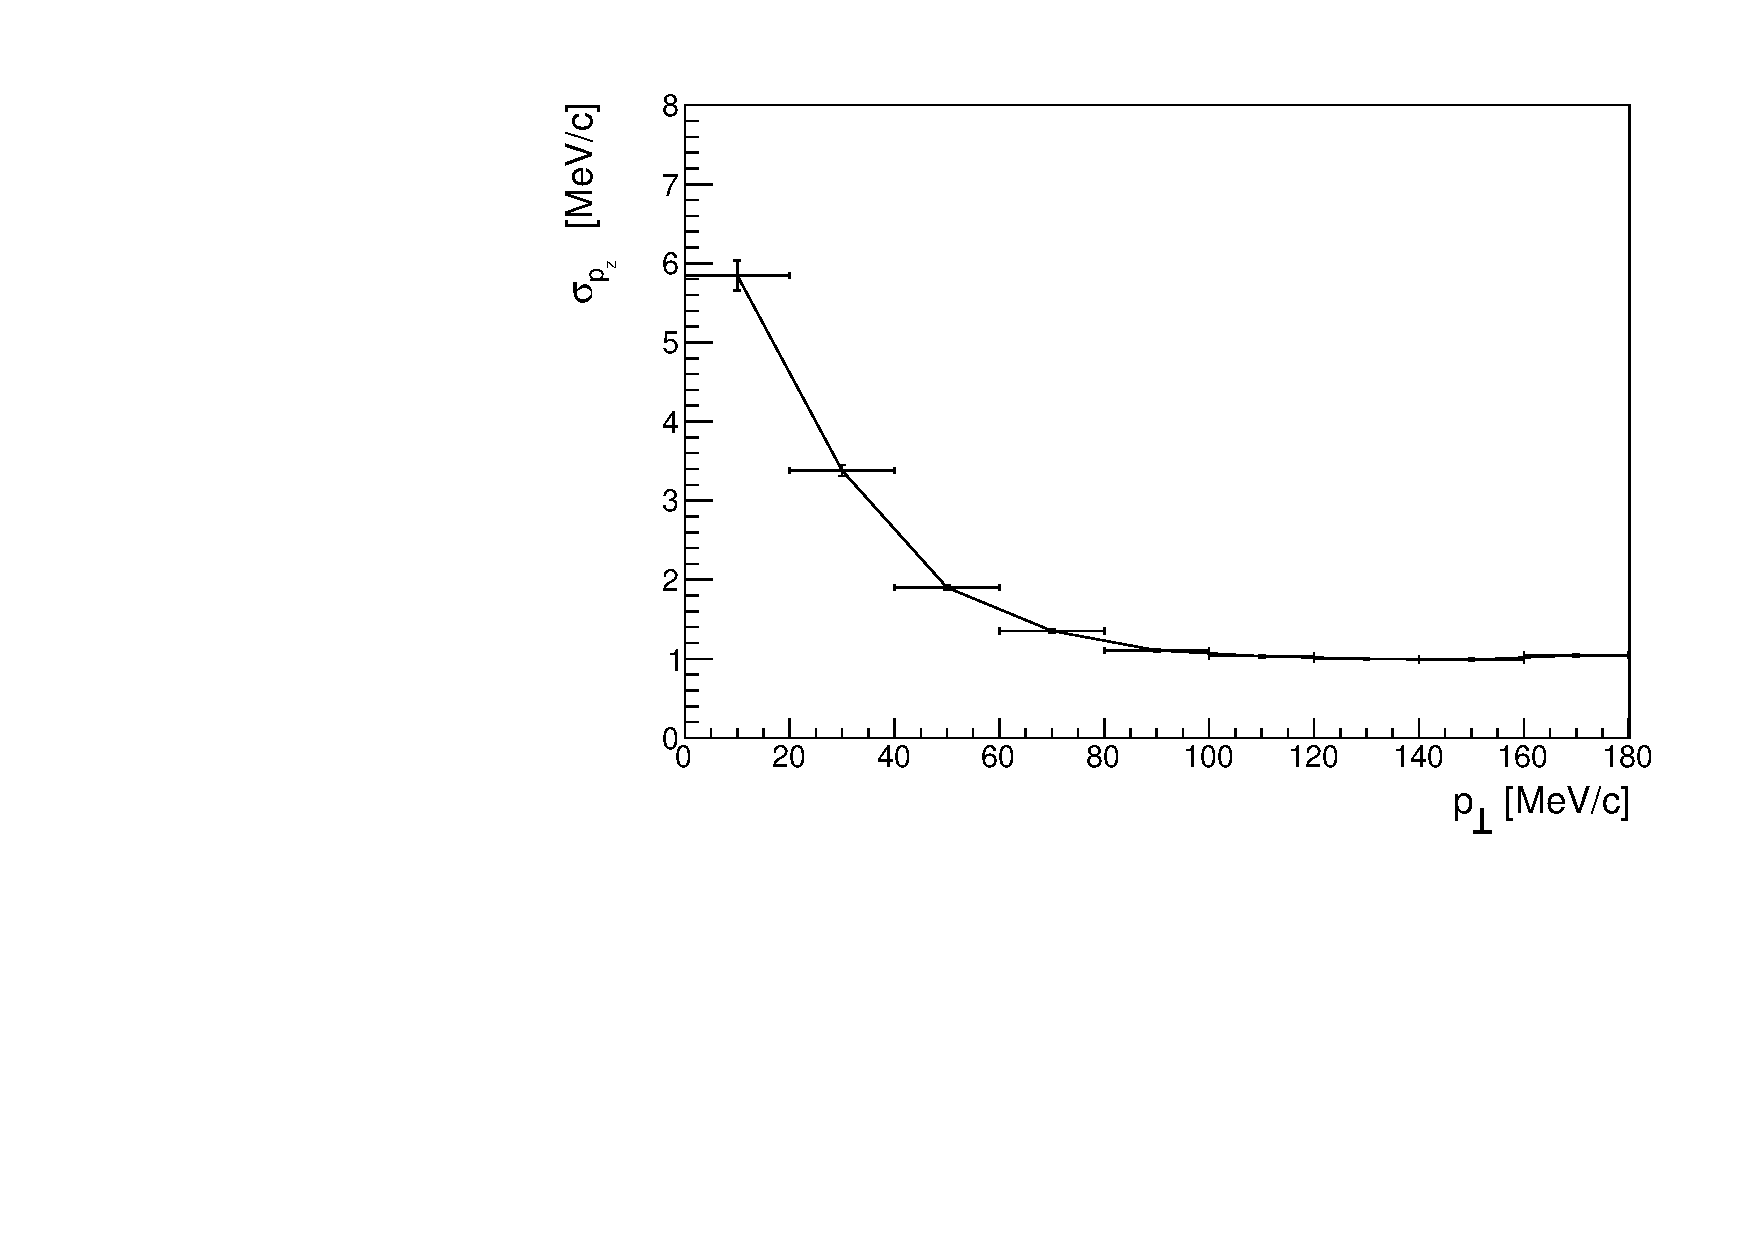
\includegraphics[width=0.49\textwidth, angle=0]{08-Performance/upstream_pz_resolution_pt.pdf}
     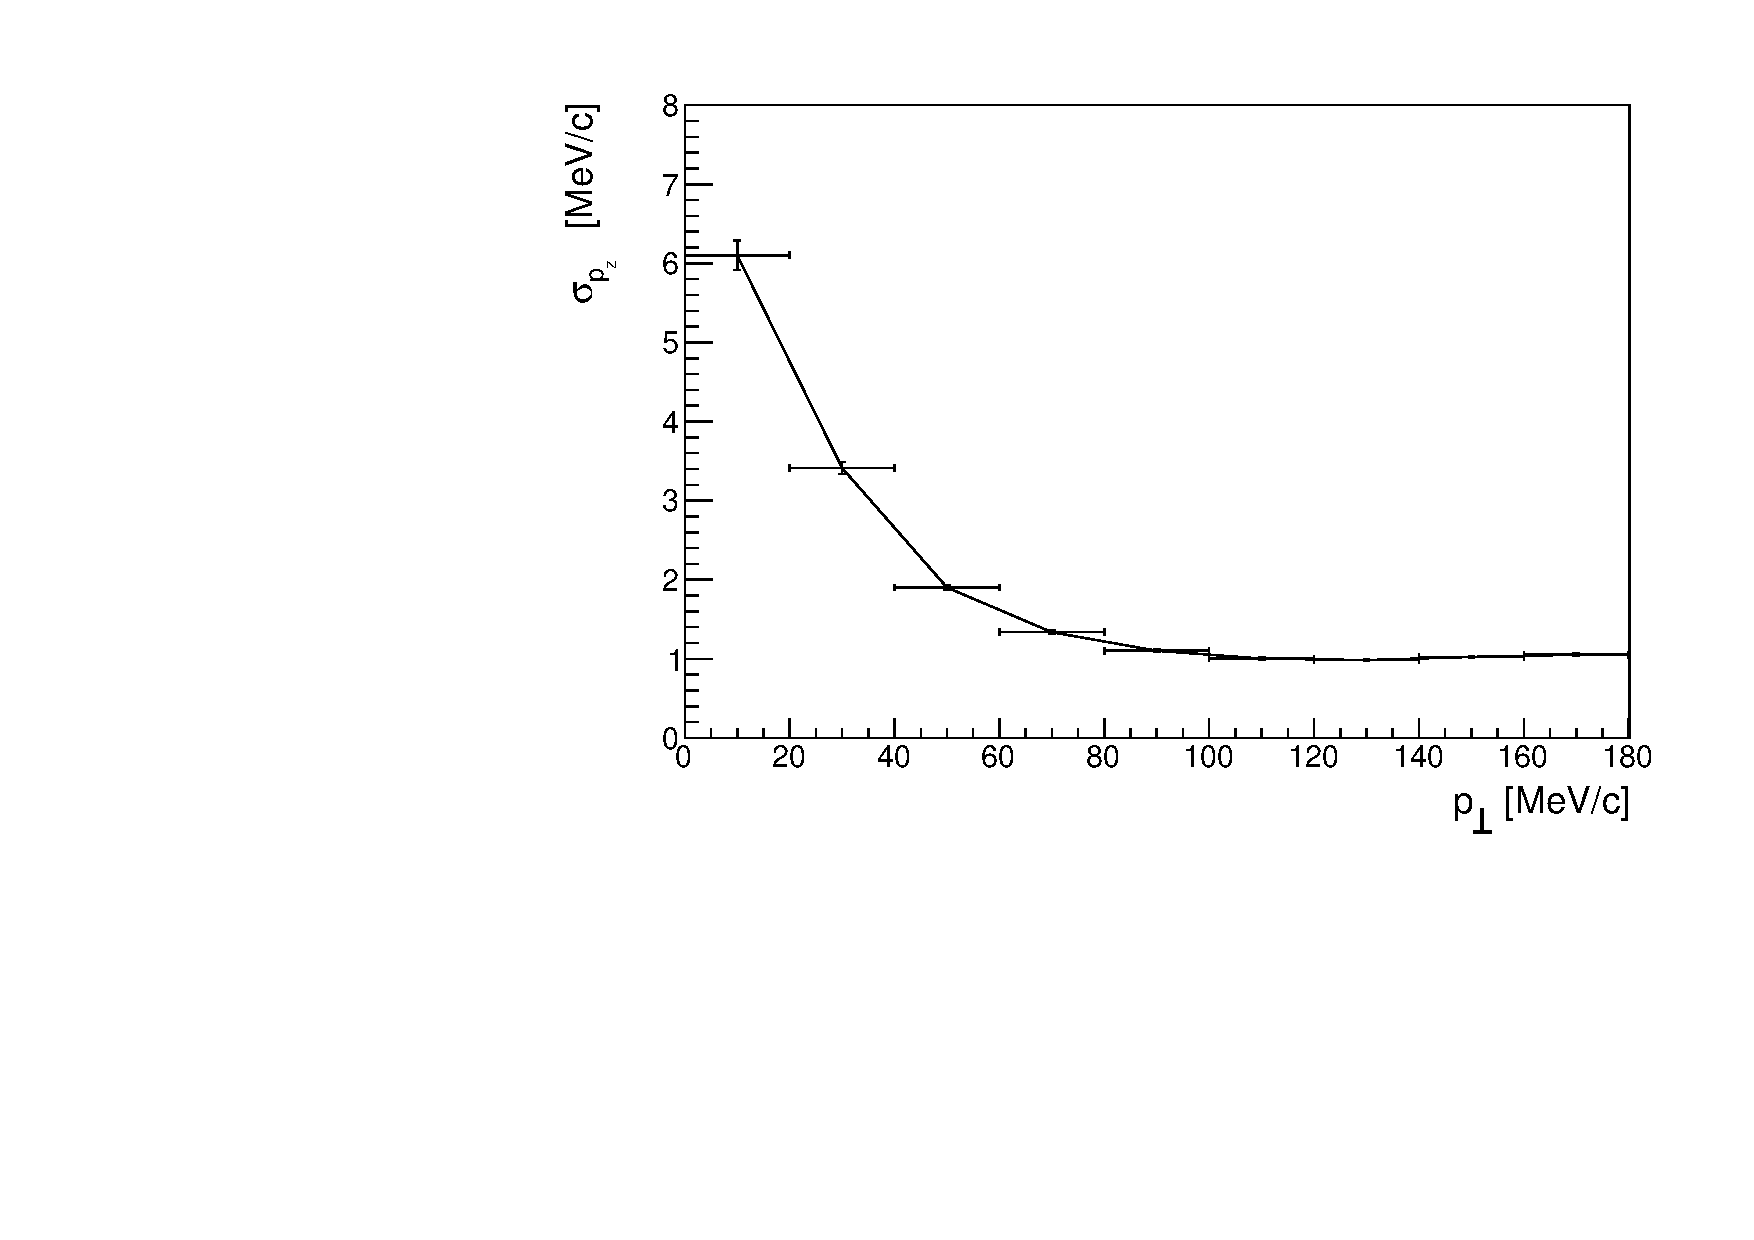
\includegraphics[width=0.49\textwidth, angle=0]{08-Performance/downstream_pz_resolution_pt.pdf}
     \caption{\label{fig:PtPzResolKalman} The $p_z$ resolution vs the $p_{\perp}$ of the upstream (left) and downstream (right).}
   \end{center}
  \end{figure}
